\documentclass[twoside]{book}

% Packages required by doxygen
\usepackage{calc}
\usepackage{doxygen}
\usepackage{graphicx}
\usepackage[utf8]{inputenc}
\usepackage{makeidx}
\usepackage{multicol}
\usepackage{multirow}
\usepackage{textcomp}
\usepackage[table]{xcolor}

% Font selection
\usepackage[T1]{fontenc}
\usepackage{mathptmx}
\usepackage[scaled=.90]{helvet}
\usepackage{courier}
\usepackage{amssymb}
\usepackage{sectsty}
\renewcommand{\familydefault}{\sfdefault}
\allsectionsfont{%
  \fontseries{bc}\selectfont%
  \color{darkgray}%
}
\renewcommand{\DoxyLabelFont}{%
  \fontseries{bc}\selectfont%
  \color{darkgray}%
}

% Page & text layout
\usepackage{geometry}
\geometry{%
  a4paper,%
  top=2.5cm,%
  bottom=2.5cm,%
  left=2.5cm,%
  right=2.5cm%
}
\tolerance=750
\hfuzz=15pt
\hbadness=750
\setlength{\emergencystretch}{15pt}
\setlength{\parindent}{0cm}
\setlength{\parskip}{0.2cm}
\makeatletter
\renewcommand{\paragraph}{%
  \@startsection{paragraph}{4}{0ex}{-1.0ex}{1.0ex}{%
    \normalfont\normalsize\bfseries\SS@parafont%
  }%
}
\renewcommand{\subparagraph}{%
  \@startsection{subparagraph}{5}{0ex}{-1.0ex}{1.0ex}{%
    \normalfont\normalsize\bfseries\SS@subparafont%
  }%
}
\makeatother

% Headers & footers
\usepackage{fancyhdr}
\pagestyle{fancyplain}
\fancyhead[LE]{\fancyplain{}{\bfseries\thepage}}
\fancyhead[CE]{\fancyplain{}{}}
\fancyhead[RE]{\fancyplain{}{\bfseries\leftmark}}
\fancyhead[LO]{\fancyplain{}{\bfseries\rightmark}}
\fancyhead[CO]{\fancyplain{}{}}
\fancyhead[RO]{\fancyplain{}{\bfseries\thepage}}
\fancyfoot[LE]{\fancyplain{}{}}
\fancyfoot[CE]{\fancyplain{}{}}
\fancyfoot[RE]{\fancyplain{}{\bfseries\scriptsize Generated on Mon May 15 2017 20\-:48\-:24 for perfect\-Parts by Doxygen }}
\fancyfoot[LO]{\fancyplain{}{\bfseries\scriptsize Generated on Mon May 15 2017 20\-:48\-:24 for perfect\-Parts by Doxygen }}
\fancyfoot[CO]{\fancyplain{}{}}
\fancyfoot[RO]{\fancyplain{}{}}
\renewcommand{\footrulewidth}{0.4pt}
\renewcommand{\chaptermark}[1]{%
  \markboth{#1}{}%
}
\renewcommand{\sectionmark}[1]{%
  \markright{\thesection\ #1}%
}

% Indices & bibliography
\usepackage{natbib}
\usepackage[titles]{tocloft}
\setcounter{tocdepth}{3}
\setcounter{secnumdepth}{5}
\makeindex

% Hyperlinks (required, but should be loaded last)
\usepackage{ifpdf}
\ifpdf
  \usepackage[pdftex,pagebackref=true]{hyperref}
\else
  \usepackage[ps2pdf,pagebackref=true]{hyperref}
\fi
\hypersetup{%
  colorlinks=true,%
  linkcolor=blue,%
  citecolor=blue,%
  unicode%
}

% Custom commands
\newcommand{\clearemptydoublepage}{%
  \newpage{\pagestyle{empty}\cleardoublepage}%
}


%===== C O N T E N T S =====

\begin{document}

% Titlepage & ToC
\hypersetup{pageanchor=false}
\pagenumbering{roman}
\begin{titlepage}
\vspace*{7cm}
\begin{center}%
{\Large perfect\-Parts }\\
\vspace*{1cm}
{\large Generated by Doxygen 1.8.5}\\
\vspace*{0.5cm}
{\small Mon May 15 2017 20:48:24}\\
\end{center}
\end{titlepage}
\clearemptydoublepage
\tableofcontents
\clearemptydoublepage
\pagenumbering{arabic}
\hypersetup{pageanchor=true}

%--- Begin generated contents ---
\chapter{Todo List}
\label{todo}
\hypertarget{todo}{}

\begin{DoxyRefList}
\item[\label{todo__todo000001}%
\hypertarget{todo__todo000001}{}%
Class \hyperlink{classEmitter}{Emitter} ]add more variables for gui  
\item[\label{todo__todo000002}%
\hypertarget{todo__todo000002}{}%
Class \hyperlink{classScene}{Scene} ]extend G\-U\-I functionality 
\end{DoxyRefList}
\chapter{Hierarchical Index}
\section{Class Hierarchy}
This inheritance list is sorted roughly, but not completely, alphabetically\-:\begin{DoxyCompactList}
\item \contentsline{section}{Emitter}{\pageref{classEmitter}}{}
\item \contentsline{section}{Particle}{\pageref{classParticle}}{}
\begin{DoxyCompactList}
\item \contentsline{section}{Explosion\-Particle}{\pageref{classExplosionParticle}}{}
\item \contentsline{section}{Firework\-Particle}{\pageref{classFireworkParticle}}{}
\item \contentsline{section}{Flame\-Particle}{\pageref{classFlameParticle}}{}
\end{DoxyCompactList}
\item \contentsline{section}{Scene}{\pageref{classScene}}{}
\end{DoxyCompactList}

\chapter{Class Index}
\section{Class List}
Here are the classes, structs, unions and interfaces with brief descriptions\-:\begin{DoxyCompactList}
\item\contentsline{section}{\hyperlink{classEmitter}{Emitter} \\*Encapsulates a particle emitter }{\pageref{classEmitter}}{}
\item\contentsline{section}{\hyperlink{classExplosionParticle}{Explosion\-Particle} \\*Encapsulates an explosion particle, is derived from abstract \hyperlink{classParticle}{Particle} class }{\pageref{classExplosionParticle}}{}
\item\contentsline{section}{\hyperlink{classFireworkParticle}{Firework\-Particle} \\*Encapsulates a firework particle, is derived from abstract \hyperlink{classParticle}{Particle} class }{\pageref{classFireworkParticle}}{}
\item\contentsline{section}{\hyperlink{classFlameParticle}{Flame\-Particle} \\*Encapsulates a flame particle, is derived from abstract \hyperlink{classParticle}{Particle} class }{\pageref{classFlameParticle}}{}
\item\contentsline{section}{\hyperlink{classParticle}{Particle} \\*Encapsulates a particle }{\pageref{classParticle}}{}
\item\contentsline{section}{\hyperlink{classScene}{Scene} \\*Encapsulates a 3\-D Open\-G\-L \hyperlink{classScene}{Scene} }{\pageref{classScene}}{}
\end{DoxyCompactList}

\chapter{File Index}
\section{File List}
Here is a list of all documented files with brief descriptions\-:\begin{DoxyCompactList}
\item\contentsline{section}{include/\hyperlink{Emitter_8h}{Emitter.\-h} }{\pageref{Emitter_8h}}{}
\item\contentsline{section}{include/\hyperlink{ExplosionParticle_8h}{Explosion\-Particle.\-h} }{\pageref{ExplosionParticle_8h}}{}
\item\contentsline{section}{include/\hyperlink{FireworkParticle_8h}{Firework\-Particle.\-h} }{\pageref{FireworkParticle_8h}}{}
\item\contentsline{section}{include/\hyperlink{FlameParticle_8h}{Flame\-Particle.\-h} }{\pageref{FlameParticle_8h}}{}
\item\contentsline{section}{include/\hyperlink{Particle_8h}{Particle.\-h} }{\pageref{Particle_8h}}{}
\item\contentsline{section}{include/\hyperlink{pngutils_8h}{pngutils.\-h} }{\pageref{pngutils_8h}}{}
\item\contentsline{section}{include/\hyperlink{Scene_8h}{Scene.\-h} }{\pageref{Scene_8h}}{}
\item\contentsline{section}{src/\hyperlink{Emitter_8cpp}{Emitter.\-cpp} \\*Implementation files for \hyperlink{classEmitter}{Emitter} class }{\pageref{Emitter_8cpp}}{}
\item\contentsline{section}{src/\hyperlink{ExplosionParticle_8cpp}{Explosion\-Particle.\-cpp} \\*Implementation files for Explosion \hyperlink{classParticle}{Particle} class }{\pageref{ExplosionParticle_8cpp}}{}
\item\contentsline{section}{src/\hyperlink{FireworkParticle_8cpp}{Firework\-Particle.\-cpp} \\*Implementation files for Firework \hyperlink{classParticle}{Particle} class }{\pageref{FireworkParticle_8cpp}}{}
\item\contentsline{section}{src/\hyperlink{main_8cpp}{main.\-cpp} \\*Main function }{\pageref{main_8cpp}}{}
\item\contentsline{section}{src/\hyperlink{Particle_8cpp}{Particle.\-cpp} \\*Implementation files for \hyperlink{classParticle}{Particle} class }{\pageref{Particle_8cpp}}{}
\end{DoxyCompactList}

\chapter{Class Documentation}
\hypertarget{classEmitter}{\section{Emitter Class Reference}
\label{classEmitter}\index{Emitter@{Emitter}}
}


encapsulates a particle emitter  




{\ttfamily \#include $<$Emitter.\-h$>$}

\subsection*{Public Member Functions}
\begin{DoxyCompactItemize}
\item 
\hypertarget{classEmitter_ab3e306b6807f4113b77e0f0dc402f8ee}{\hyperlink{classEmitter_ab3e306b6807f4113b77e0f0dc402f8ee}{Emitter} ()=default}\label{classEmitter_ab3e306b6807f4113b77e0f0dc402f8ee}

\begin{DoxyCompactList}\small\item\em Default constructor that initialises member variables to default values. \end{DoxyCompactList}\item 
\hyperlink{classEmitter_a441e3b9302f39f0d359773e5ed72afb7}{Emitter} (glm\-::vec3 const \&\-\_\-pos, size\-\_\-t const \&\-\_\-max)
\begin{DoxyCompactList}\small\item\em Constructor using a passed position and particle limit. \end{DoxyCompactList}\item 
\hypertarget{classEmitter_abe9a91a6a709a244ec17c9f8284c279e}{\hyperlink{classEmitter_abe9a91a6a709a244ec17c9f8284c279e}{Emitter} (\hyperlink{classEmitter}{Emitter} const \&)=delete}\label{classEmitter_abe9a91a6a709a244ec17c9f8284c279e}

\begin{DoxyCompactList}\small\item\em Delete copy constructor, D\-O N\-O\-T I\-M\-P\-L\-E\-M\-E\-N\-T, class contains unique pointer. \end{DoxyCompactList}\item 
\hypertarget{classEmitter_a9c2eef3cc2d4909b4f8053abc2a66505}{\hyperlink{classEmitter}{Emitter} \& \hyperlink{classEmitter_a9c2eef3cc2d4909b4f8053abc2a66505}{operator=} (\hyperlink{classEmitter}{Emitter} const \&)=delete}\label{classEmitter_a9c2eef3cc2d4909b4f8053abc2a66505}

\begin{DoxyCompactList}\small\item\em Delete assignment, D\-O N\-O\-T I\-M\-P\-L\-E\-M\-E\-N\-T, class contains unique pointer. \end{DoxyCompactList}\item 
\hypertarget{classEmitter_a0af9a50316daf2580cde9b99fe7c6f96}{\hyperlink{classEmitter_a0af9a50316daf2580cde9b99fe7c6f96}{$\sim$\-Emitter} ()}\label{classEmitter_a0af9a50316daf2580cde9b99fe7c6f96}

\begin{DoxyCompactList}\small\item\em Default destructor. \end{DoxyCompactList}\item 
void \hyperlink{classEmitter_a9fbfc0ce29b00564ff2366aa4c9e10af}{init\-Texture} (G\-Luint $\ast$const \&o\-\_\-tex, std\-::string const \&\-\_\-tex\-Path) const 
\begin{DoxyCompactList}\small\item\em Initialises textures at the provided filepath. \end{DoxyCompactList}\item 
\hypertarget{classEmitter_a2ece709498f9cbbb9d4f8cba2780b0e9}{void \hyperlink{classEmitter_a2ece709498f9cbbb9d4f8cba2780b0e9}{update} ()}\label{classEmitter_a2ece709498f9cbbb9d4f8cba2780b0e9}

\begin{DoxyCompactList}\small\item\em Updates all particles in the system. \end{DoxyCompactList}\item 
\hypertarget{classEmitter_ad0ef8fd3cc8a6d1b8996ec8da041e967}{void \hyperlink{classEmitter_ad0ef8fd3cc8a6d1b8996ec8da041e967}{draw} () const }\label{classEmitter_ad0ef8fd3cc8a6d1b8996ec8da041e967}

\begin{DoxyCompactList}\small\item\em Draws all particles in the system. \end{DoxyCompactList}\item 
\hypertarget{classEmitter_a4b7046dbc627e71f29dbbb17b3ea0415}{std\-::size\-\_\-t \hyperlink{classEmitter_a4b7046dbc627e71f29dbbb17b3ea0415}{particle\-Count} () const }\label{classEmitter_a4b7046dbc627e71f29dbbb17b3ea0415}

\begin{DoxyCompactList}\small\item\em Returns the current amount of particles in the system. \end{DoxyCompactList}\item 
\hypertarget{classEmitter_a64b6f240ca3d13e60789d92bbfe4d517}{std\-::size\-\_\-t \hyperlink{classEmitter_a64b6f240ca3d13e60789d92bbfe4d517}{max\-Particles} () const }\label{classEmitter_a64b6f240ca3d13e60789d92bbfe4d517}

\begin{DoxyCompactList}\small\item\em Returns the maximum number of particles allowed to be in the system. \end{DoxyCompactList}\item 
\hypertarget{classEmitter_a4320b2c9aff78bc6fbb318b320291f6f}{std\-::size\-\_\-t \hyperlink{classEmitter_a4320b2c9aff78bc6fbb318b320291f6f}{vector\-Size} () const }\label{classEmitter_a4320b2c9aff78bc6fbb318b320291f6f}

\begin{DoxyCompactList}\small\item\em Returns the current size of the array. \end{DoxyCompactList}\item 
\hypertarget{classEmitter_a8d3c4dba0d12c1952350cbc4cda69db7}{glm\-::vec3 \hyperlink{classEmitter_a8d3c4dba0d12c1952350cbc4cda69db7}{pos} () const }\label{classEmitter_a8d3c4dba0d12c1952350cbc4cda69db7}

\begin{DoxyCompactList}\small\item\em Returns the current position. \end{DoxyCompactList}\item 
void \hyperlink{classEmitter_a6229955278657909f2f88731d5015118}{set\-Pos} (glm\-::vec3 const \&\-\_\-pos)
\begin{DoxyCompactList}\small\item\em Sets the current position to the provided position. \end{DoxyCompactList}\item 
void \hyperlink{classEmitter_aa8ee7a71384a6759b675188221630f1a}{set\-Max\-Particles} (size\-\_\-t const \&\-\_\-max)
\begin{DoxyCompactList}\small\item\em Sets the particle limit to the provided size provided. \end{DoxyCompactList}\end{DoxyCompactItemize}
\subsection*{Public Attributes}
\begin{DoxyCompactItemize}
\item 
\hypertarget{classEmitter_a1cecbc82f0907e305afb6d6a4d6a3021}{bool \hyperlink{classEmitter_a1cecbc82f0907e305afb6d6a4d6a3021}{m\-\_\-reduce\-Memory} = false}\label{classEmitter_a1cecbc82f0907e305afb6d6a4d6a3021}

\begin{DoxyCompactList}\small\item\em Flag used to determine whether the emitter should clear dead particles from m\-\_\-particles when unused, this will save memory but could slow down the system. \end{DoxyCompactList}\item 
\hypertarget{classEmitter_a24c3fe59e6f1ac64d61a9681d7a6c943}{bool \hyperlink{classEmitter_a24c3fe59e6f1ac64d61a9681d7a6c943}{m\-\_\-flame} = false}\label{classEmitter_a24c3fe59e6f1ac64d61a9681d7a6c943}

\begin{DoxyCompactList}\small\item\em Flag used to spawn flame into the system. \end{DoxyCompactList}\item 
\hypertarget{classEmitter_acd5d5ce9370f9e45d73ec7182155ad69}{glm\-::vec4 \hyperlink{classEmitter_acd5d5ce9370f9e45d73ec7182155ad69}{m\-\_\-fl\-Col} = glm\-::vec4(1.\-0f,0.\-67f,0.\-0f,1.\-0f)}\label{classEmitter_acd5d5ce9370f9e45d73ec7182155ad69}

\begin{DoxyCompactList}\small\item\em Colour that the new flame will be. \end{DoxyCompactList}\item 
\hypertarget{classEmitter_a7835d97db9ca64b7534eba110e0f7845}{float \hyperlink{classEmitter_a7835d97db9ca64b7534eba110e0f7845}{m\-\_\-fl\-Speed} = 1.\-2f}\label{classEmitter_a7835d97db9ca64b7534eba110e0f7845}

\begin{DoxyCompactList}\small\item\em Speed of the flame. \end{DoxyCompactList}\item 
\hypertarget{classEmitter_a4e024aa6c38ea9eb95c076d2325e0dfe}{int \hyperlink{classEmitter_a4e024aa6c38ea9eb95c076d2325e0dfe}{m\-\_\-fl\-Life} = 40}\label{classEmitter_a4e024aa6c38ea9eb95c076d2325e0dfe}

\begin{DoxyCompactList}\small\item\em Average life of flame particles. \end{DoxyCompactList}\item 
\hypertarget{classEmitter_a56f401933d8c66a8355e9d3073041311}{int \hyperlink{classEmitter_a56f401933d8c66a8355e9d3073041311}{m\-\_\-fl\-Density} = 10}\label{classEmitter_a56f401933d8c66a8355e9d3073041311}

\begin{DoxyCompactList}\small\item\em Amount of spawning particles to add every frame. \end{DoxyCompactList}\item 
\hypertarget{classEmitter_a77f3919bf2449d9fe9ab2294d824a10b}{float \hyperlink{classEmitter_a77f3919bf2449d9fe9ab2294d824a10b}{m\-\_\-fl\-Spread} = 2.\-0f}\label{classEmitter_a77f3919bf2449d9fe9ab2294d824a10b}

\begin{DoxyCompactList}\small\item\em Spread of intial flame particle positions. \end{DoxyCompactList}\item 
\hypertarget{classEmitter_a254bbe70cc78563bc3e035eaa594c82d}{float \hyperlink{classEmitter_a254bbe70cc78563bc3e035eaa594c82d}{m\-\_\-fl\-Steepness} = 0.\-26f}\label{classEmitter_a254bbe70cc78563bc3e035eaa594c82d}

\begin{DoxyCompactList}\small\item\em \hyperlink{classEmitter}{Emitter} angle for the flame particles. \end{DoxyCompactList}\item 
\hypertarget{classEmitter_ab44f6794ae404bc2a6885f968241fa87}{float \hyperlink{classEmitter_ab44f6794ae404bc2a6885f968241fa87}{m\-\_\-fl\-Size} = 120.\-0f}\label{classEmitter_ab44f6794ae404bc2a6885f968241fa87}

\begin{DoxyCompactList}\small\item\em \hyperlink{classEmitter}{Emitter} angle for the flame particles. \end{DoxyCompactList}\item 
\hypertarget{classEmitter_aad0ffc2fadafa73475b9310ef57822f3}{bool \hyperlink{classEmitter_aad0ffc2fadafa73475b9310ef57822f3}{m\-\_\-fl\-Children} = true}\label{classEmitter_aad0ffc2fadafa73475b9310ef57822f3}

\begin{DoxyCompactList}\small\item\em \hyperlink{classEmitter}{Emitter} angle for the flame particles. \end{DoxyCompactList}\item 
\hypertarget{classEmitter_a4e6f9266ac19bf3d185d30284bc43b24}{bool \hyperlink{classEmitter_a4e6f9266ac19bf3d185d30284bc43b24}{m\-\_\-firework} = false}\label{classEmitter_a4e6f9266ac19bf3d185d30284bc43b24}

\begin{DoxyCompactList}\small\item\em Flag used to spawn a firework into the system. \end{DoxyCompactList}\item 
\hypertarget{classEmitter_ad198e73134d1764f120e7e76acf3588b}{glm\-::vec4 \hyperlink{classEmitter_ad198e73134d1764f120e7e76acf3588b}{m\-\_\-fw\-Col} = glm\-::vec4(1.\-0f,0.\-078f,0.\-576f,1.\-0f)}\label{classEmitter_ad198e73134d1764f120e7e76acf3588b}

\begin{DoxyCompactList}\small\item\em Colour of the new firework. \end{DoxyCompactList}\item 
\hypertarget{classEmitter_a37991f5de30d840af13e253b72ea281e}{bool \hyperlink{classEmitter_a37991f5de30d840af13e253b72ea281e}{m\-\_\-fw\-Blink} = false}\label{classEmitter_a37991f5de30d840af13e253b72ea281e}

\begin{DoxyCompactList}\small\item\em Flag used to make new firework blink. \end{DoxyCompactList}\item 
\hypertarget{classEmitter_aa661616d478f33efea14b12add2d13d3}{float \hyperlink{classEmitter_aa661616d478f33efea14b12add2d13d3}{m\-\_\-fw\-Rotation} = 0.\-0f}\label{classEmitter_aa661616d478f33efea14b12add2d13d3}

\begin{DoxyCompactList}\small\item\em Angle of steepness between -\/180 and 180 degrees, that firework is ejected. \end{DoxyCompactList}\item 
\hypertarget{classEmitter_a37cf901dd5727584ee318d228abb9f94}{float \hyperlink{classEmitter_a37cf901dd5727584ee318d228abb9f94}{m\-\_\-fw\-Incline} = 0.\-0f}\label{classEmitter_a37cf901dd5727584ee318d228abb9f94}

\begin{DoxyCompactList}\small\item\em Angle of rotation between 0 and 360 degrees, that firework is ejected. \end{DoxyCompactList}\item 
\hypertarget{classEmitter_ac1325204ad2906d835790453b810763b}{float \hyperlink{classEmitter_ac1325204ad2906d835790453b810763b}{m\-\_\-fw\-Thrust} = 1.\-0f}\label{classEmitter_ac1325204ad2906d835790453b810763b}

\begin{DoxyCompactList}\small\item\em Initial velocity of firework. \end{DoxyCompactList}\item 
\hypertarget{classEmitter_adcdc6f5ca0e589fbf20ec45140c5a4aa}{int \hyperlink{classEmitter_adcdc6f5ca0e589fbf20ec45140c5a4aa}{m\-\_\-fw\-Fuel} = 300}\label{classEmitter_adcdc6f5ca0e589fbf20ec45140c5a4aa}

\begin{DoxyCompactList}\small\item\em Amount of spawning particles in firework. \end{DoxyCompactList}\item 
\hypertarget{classEmitter_a2ddd6ee2e0e1609024903644f61543fc}{int \hyperlink{classEmitter_a2ddd6ee2e0e1609024903644f61543fc}{m\-\_\-fw\-Trail} = 20}\label{classEmitter_a2ddd6ee2e0e1609024903644f61543fc}

\begin{DoxyCompactList}\small\item\em Lifespan of firework trail particles. \end{DoxyCompactList}\item 
\hypertarget{classEmitter_ab17edfb3652261eb28b1d03f91f9d044}{int \hyperlink{classEmitter_ab17edfb3652261eb28b1d03f91f9d044}{m\-\_\-fw\-Fuse} = 95}\label{classEmitter_ab17edfb3652261eb28b1d03f91f9d044}

\begin{DoxyCompactList}\small\item\em Fuse timer in frames before firework explodes. \end{DoxyCompactList}\item 
\hypertarget{classEmitter_a4b411dc3c9945ce1b987e67dfe73034d}{int \hyperlink{classEmitter_a4b411dc3c9945ce1b987e67dfe73034d}{m\-\_\-fw\-Exp\-Life} = 80}\label{classEmitter_a4b411dc3c9945ce1b987e67dfe73034d}

\begin{DoxyCompactList}\small\item\em Lifespan of spawning particles in firework after explosion. \end{DoxyCompactList}\item 
\hypertarget{classEmitter_ad4f37d42386349dd35897d1f90bc9626}{int \hyperlink{classEmitter_ad4f37d42386349dd35897d1f90bc9626}{m\-\_\-explosions} = 0}\label{classEmitter_ad4f37d42386349dd35897d1f90bc9626}

\begin{DoxyCompactList}\small\item\em We detonate explosions over multiple frames to simulate a chain explosion, this give a more realistic look, this variable holds the remaining number of frames for which we will detonate explosions. \end{DoxyCompactList}\item 
\hypertarget{classEmitter_a2fb204e6cb07011468d7603f7aa8bce7}{glm\-::vec4 \hyperlink{classEmitter_a2fb204e6cb07011468d7603f7aa8bce7}{m\-\_\-exp\-Col} = glm\-::vec4(0.\-647f,0.\-306f,0.\-2f,1.\-0f)}\label{classEmitter_a2fb204e6cb07011468d7603f7aa8bce7}

\begin{DoxyCompactList}\small\item\em Colour of new explosion. \end{DoxyCompactList}\item 
\hypertarget{classEmitter_a0e8ab9310a04b5860722e3cb953642e6}{int \hyperlink{classEmitter_a0e8ab9310a04b5860722e3cb953642e6}{m\-\_\-exp\-Density} = 20}\label{classEmitter_a0e8ab9310a04b5860722e3cb953642e6}

\begin{DoxyCompactList}\small\item\em The life span of new explosion particles. \end{DoxyCompactList}\item 
\hypertarget{classEmitter_afc994081ef53be0a63ef421697844524}{int \hyperlink{classEmitter_afc994081ef53be0a63ef421697844524}{m\-\_\-exp\-Life} = 80}\label{classEmitter_afc994081ef53be0a63ef421697844524}

\begin{DoxyCompactList}\small\item\em The amount of shooting particles in the explosion. \end{DoxyCompactList}\item 
\hypertarget{classEmitter_a9698c6471e3d28a10c6210ecd2804f3d}{float \hyperlink{classEmitter_a9698c6471e3d28a10c6210ecd2804f3d}{m\-\_\-exp\-Size} = 70.\-0f}\label{classEmitter_a9698c6471e3d28a10c6210ecd2804f3d}

\begin{DoxyCompactList}\small\item\em The size of the explosion particles. \end{DoxyCompactList}\item 
\hypertarget{classEmitter_adf82b76b44887e822b839e580894a622}{float \hyperlink{classEmitter_adf82b76b44887e822b839e580894a622}{m\-\_\-exp\-Incline} = 1.\-5f}\label{classEmitter_adf82b76b44887e822b839e580894a622}

\begin{DoxyCompactList}\small\item\em The range for the explosion particle emission. \end{DoxyCompactList}\item 
\hypertarget{classEmitter_aefb05cb4e4750257404580f0792679d2}{float \hyperlink{classEmitter_aefb05cb4e4750257404580f0792679d2}{m\-\_\-exp\-Speed} = 1.\-0f}\label{classEmitter_aefb05cb4e4750257404580f0792679d2}

\begin{DoxyCompactList}\small\item\em The speed of the explosion particles. \end{DoxyCompactList}\item 
\hypertarget{classEmitter_a60ab680e86688dd4f0f428b6d88f5f06}{bool \hyperlink{classEmitter_a60ab680e86688dd4f0f428b6d88f5f06}{m\-\_\-clear} = false}\label{classEmitter_a60ab680e86688dd4f0f428b6d88f5f06}

\begin{DoxyCompactList}\small\item\em Flag to clear the system. \end{DoxyCompactList}\item 
\hypertarget{classEmitter_a79ec38b927d82009c22199a4cbecfd85}{glm\-::mat4 \hyperlink{classEmitter_a79ec38b927d82009c22199a4cbecfd85}{m\-\_\-transform} = glm\-::mat4(1.\-0f)}\label{classEmitter_a79ec38b927d82009c22199a4cbecfd85}

\begin{DoxyCompactList}\small\item\em Local transformations of the system are stored in this matrix and used for drawing. \end{DoxyCompactList}\item 
\hypertarget{classEmitter_a4530f4a730e651511dfee30293e666ba}{G\-Luint $\ast$ \hyperlink{classEmitter_a4530f4a730e651511dfee30293e666ba}{m\-\_\-textures} = new G\-Luint\mbox{[}3\mbox{]}}\label{classEmitter_a4530f4a730e651511dfee30293e666ba}

\begin{DoxyCompactList}\small\item\em Array of Open\-G\-L textures to use for our point sprites, must change the array size to add texture. \end{DoxyCompactList}\end{DoxyCompactItemize}


\subsection{Detailed Description}
encapsulates a particle emitter 

Revision History\-: See \char`\"{}https\-://github.\-com/nitronoid/perfect\-Parts\char`\"{} Initial Version 20/03/17 \begin{DoxyRefDesc}{Todo}
\item[\hyperlink{todo__todo000001}{Todo}]add more variables for gui \end{DoxyRefDesc}


\subsection{Constructor \& Destructor Documentation}
\hypertarget{classEmitter_a441e3b9302f39f0d359773e5ed72afb7}{\index{Emitter@{Emitter}!Emitter@{Emitter}}
\index{Emitter@{Emitter}!Emitter@{Emitter}}
\subsubsection[{Emitter}]{\setlength{\rightskip}{0pt plus 5cm}Emitter\-::\-Emitter (
\begin{DoxyParamCaption}
\item[{glm\-::vec3 const \&}]{\-\_\-pos, }
\item[{size\-\_\-t const \&}]{\-\_\-max}
\end{DoxyParamCaption}
)}}\label{classEmitter_a441e3b9302f39f0d359773e5ed72afb7}


Constructor using a passed position and particle limit. 


\begin{DoxyParams}[1]{Parameters}
\mbox{\tt in}  & {\em \-\_\-pos} & the position of the emitter \\
\hline
\mbox{\tt in}  & {\em \-\_\-max} & the particle limit \\
\hline
\end{DoxyParams}


\subsection{Member Function Documentation}
\hypertarget{classEmitter_a9fbfc0ce29b00564ff2366aa4c9e10af}{\index{Emitter@{Emitter}!init\-Texture@{init\-Texture}}
\index{init\-Texture@{init\-Texture}!Emitter@{Emitter}}
\subsubsection[{init\-Texture}]{\setlength{\rightskip}{0pt plus 5cm}void Emitter\-::init\-Texture (
\begin{DoxyParamCaption}
\item[{G\-Luint $\ast$const \&}]{o\-\_\-tex, }
\item[{std\-::string const \&}]{\-\_\-tex\-Path}
\end{DoxyParamCaption}
) const}}\label{classEmitter_a9fbfc0ce29b00564ff2366aa4c9e10af}


Initialises textures at the provided filepath. 


\begin{DoxyParams}[1]{Parameters}
 & {\em o\mbox{]}} & o\-\_\-tex a pointer to store the open\-G\-L texture \\
\hline
\mbox{\tt in}  & {\em \-\_\-tex\-Path} & the filepath to the texture \\
\hline
\end{DoxyParams}
\hypertarget{classEmitter_aa8ee7a71384a6759b675188221630f1a}{\index{Emitter@{Emitter}!set\-Max\-Particles@{set\-Max\-Particles}}
\index{set\-Max\-Particles@{set\-Max\-Particles}!Emitter@{Emitter}}
\subsubsection[{set\-Max\-Particles}]{\setlength{\rightskip}{0pt plus 5cm}void Emitter\-::set\-Max\-Particles (
\begin{DoxyParamCaption}
\item[{size\-\_\-t const \&}]{\-\_\-max}
\end{DoxyParamCaption}
)\hspace{0.3cm}{\ttfamily [inline]}}}\label{classEmitter_aa8ee7a71384a6759b675188221630f1a}


Sets the particle limit to the provided size provided. 


\begin{DoxyParams}[1]{Parameters}
\mbox{\tt in}  & {\em \-\_\-max} & the new particle limit \\
\hline
\end{DoxyParams}
\hypertarget{classEmitter_a6229955278657909f2f88731d5015118}{\index{Emitter@{Emitter}!set\-Pos@{set\-Pos}}
\index{set\-Pos@{set\-Pos}!Emitter@{Emitter}}
\subsubsection[{set\-Pos}]{\setlength{\rightskip}{0pt plus 5cm}void Emitter\-::set\-Pos (
\begin{DoxyParamCaption}
\item[{glm\-::vec3 const \&}]{\-\_\-pos}
\end{DoxyParamCaption}
)\hspace{0.3cm}{\ttfamily [inline]}}}\label{classEmitter_a6229955278657909f2f88731d5015118}


Sets the current position to the provided position. 


\begin{DoxyParams}[1]{Parameters}
\mbox{\tt in}  & {\em \-\_\-pos} & the new position \\
\hline
\end{DoxyParams}


The documentation for this class was generated from the following files\-:\begin{DoxyCompactItemize}
\item 
include/\hyperlink{Emitter_8h}{Emitter.\-h}\item 
src/\hyperlink{Emitter_8cpp}{Emitter.\-cpp}\end{DoxyCompactItemize}

\hypertarget{classExplosionParticle}{\section{Explosion\-Particle Class Reference}
\label{classExplosionParticle}\index{Explosion\-Particle@{Explosion\-Particle}}
}


encapsulates an explosion particle, is derived from abstract \hyperlink{classParticle}{Particle} class  




{\ttfamily \#include $<$Explosion\-Particle.\-h$>$}

Inheritance diagram for Explosion\-Particle\-:\begin{figure}[H]
\begin{center}
\leavevmode
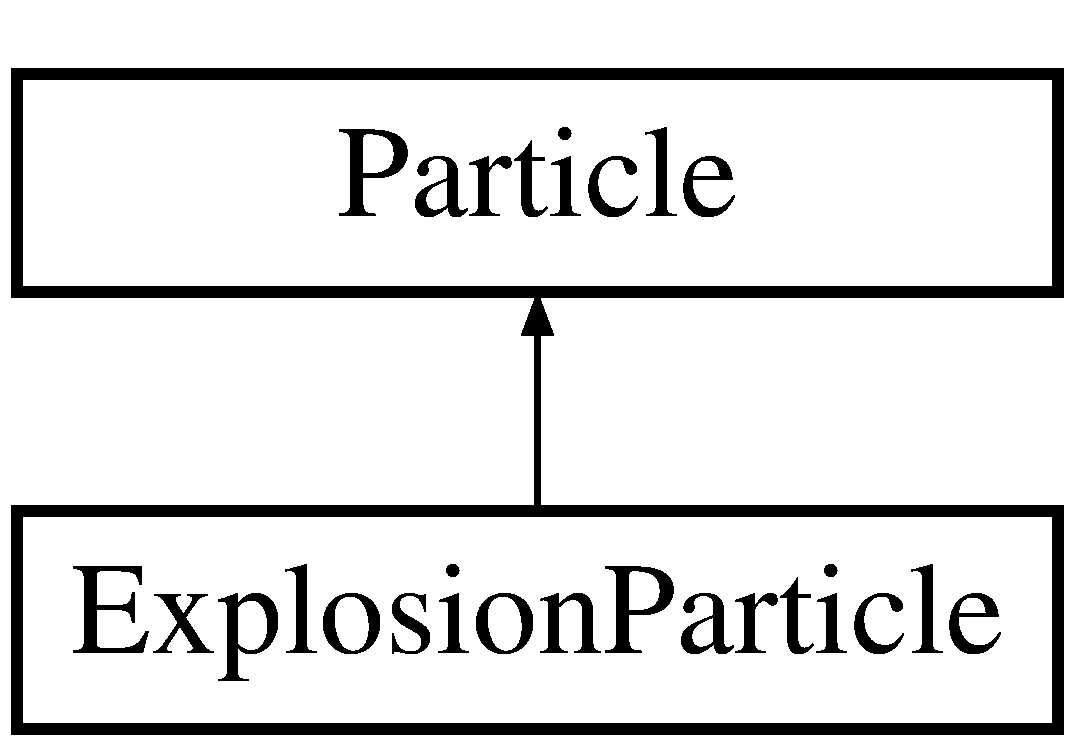
\includegraphics[height=2.000000cm]{classExplosionParticle}
\end{center}
\end{figure}
\subsection*{Public Member Functions}
\begin{DoxyCompactItemize}
\item 
\hypertarget{classExplosionParticle_a2175ab3a5622c59880a5e087ee113b43}{\hyperlink{classExplosionParticle_a2175ab3a5622c59880a5e087ee113b43}{Explosion\-Particle} ()=default}\label{classExplosionParticle_a2175ab3a5622c59880a5e087ee113b43}

\begin{DoxyCompactList}\small\item\em Default constructor that initialises member variables to default values. \end{DoxyCompactList}\item 
\hyperlink{classExplosionParticle_a1f80155f7d52d00d04c614baa55aefac}{Explosion\-Particle} (glm\-::vec3 const \&\-\_\-pos, glm\-::vec3 const \&\-\_\-vel, glm\-::vec4 const \&\-\_\-col, float const \&\-\_\-size, int const \&\-\_\-life, int const \&\-\_\-frame, bool const \&\-\_\-spawn)
\begin{DoxyCompactList}\small\item\em Constructor using intial position, velocity, colour, size, life span and a spawn flag. \end{DoxyCompactList}\item 
\hypertarget{classExplosionParticle_aeb7b8dd431a766a92442540a5b876e03}{virtual \hyperlink{classExplosionParticle_aeb7b8dd431a766a92442540a5b876e03}{$\sim$\-Explosion\-Particle} ()=default}\label{classExplosionParticle_aeb7b8dd431a766a92442540a5b876e03}

\begin{DoxyCompactList}\small\item\em Default Virtual destructor for particle, neccessary to prevent memory leak. \end{DoxyCompactList}\item 
virtual int \hyperlink{classExplosionParticle_a302953be6e09fa22437248d175906e55}{new\-Parts} (int const \&) const override
\begin{DoxyCompactList}\small\item\em Returns the amount of child particles to spawn, overrides the \hyperlink{classParticle}{Particle} class implementation. \end{DoxyCompactList}\item 
virtual void \hyperlink{classExplosionParticle_ac1c36920bf241f397c639fdaac40a9f9}{update} (int const \&\-\_\-frame) override
\begin{DoxyCompactList}\small\item\em Updates the particle properties, overrides the \hyperlink{classParticle}{Particle} class implementation. \end{DoxyCompactList}\item 
virtual \hyperlink{classParticle}{Particle} $\ast$ \hyperlink{classExplosionParticle_a1948c2b0f3b39d303b2d8cef6b0e0701}{create\-Child} (int const \&\-\_\-frame) const override
\begin{DoxyCompactList}\small\item\em Creates a pointer to a child particle, overrides the \hyperlink{classParticle}{Particle} class implementation. \end{DoxyCompactList}\item 
virtual void \hyperlink{classExplosionParticle_a0e3a9cd71e0d13732254f9184b7f38e9}{draw} (int const \&) const override
\begin{DoxyCompactList}\small\item\em Draws the particle, overrides the \hyperlink{classParticle}{Particle} class implementation. \end{DoxyCompactList}\end{DoxyCompactItemize}
\subsection*{Additional Inherited Members}


\subsection{Detailed Description}
encapsulates an explosion particle, is derived from abstract \hyperlink{classParticle}{Particle} class 

Revision History\-: See \char`\"{}https\-://github.\-com/nitronoid/perfect\-Parts\char`\"{} Initial Version 24/03/17 

\subsection{Constructor \& Destructor Documentation}
\hypertarget{classExplosionParticle_a1f80155f7d52d00d04c614baa55aefac}{\index{Explosion\-Particle@{Explosion\-Particle}!Explosion\-Particle@{Explosion\-Particle}}
\index{Explosion\-Particle@{Explosion\-Particle}!ExplosionParticle@{Explosion\-Particle}}
\subsubsection[{Explosion\-Particle}]{\setlength{\rightskip}{0pt plus 5cm}Explosion\-Particle\-::\-Explosion\-Particle (
\begin{DoxyParamCaption}
\item[{glm\-::vec3 const \&}]{\-\_\-pos, }
\item[{glm\-::vec3 const \&}]{\-\_\-vel, }
\item[{glm\-::vec4 const \&}]{\-\_\-col, }
\item[{float const \&}]{\-\_\-size, }
\item[{int const \&}]{\-\_\-life, }
\item[{int const \&}]{\-\_\-frame, }
\item[{bool const \&}]{\-\_\-spawn}
\end{DoxyParamCaption}
)}}\label{classExplosionParticle_a1f80155f7d52d00d04c614baa55aefac}


Constructor using intial position, velocity, colour, size, life span and a spawn flag. 


\begin{DoxyParams}[1]{Parameters}
\mbox{\tt in}  & {\em \-\_\-pos} & the initial position of the particle \\
\hline
\mbox{\tt in}  & {\em \-\_\-vel} & the initial velocity of the particle \\
\hline
\mbox{\tt in}  & {\em \-\_\-col} & the initial colour of the particle \\
\hline
\mbox{\tt in}  & {\em \-\_\-size} & the initial size of the particle \\
\hline
\mbox{\tt in}  & {\em \-\_\-life} & the initial life of the particle \\
\hline
\mbox{\tt in}  & {\em \-\_\-t\-Life} & the life span of child particles that compose trails \\
\hline
\mbox{\tt in}  & {\em \-\_\-frame} & the current frame, used to set m\-\_\-birth\-Frame \\
\hline
\mbox{\tt in}  & {\em \-\_\-spawn} & used to set m\-\_\-spawn, flag for spawning children \\
\hline
\end{DoxyParams}


\subsection{Member Function Documentation}
\hypertarget{classExplosionParticle_a1948c2b0f3b39d303b2d8cef6b0e0701}{\index{Explosion\-Particle@{Explosion\-Particle}!create\-Child@{create\-Child}}
\index{create\-Child@{create\-Child}!ExplosionParticle@{Explosion\-Particle}}
\subsubsection[{create\-Child}]{\setlength{\rightskip}{0pt plus 5cm}{\bf Particle} $\ast$ Explosion\-Particle\-::create\-Child (
\begin{DoxyParamCaption}
\item[{int const \&}]{\-\_\-frame}
\end{DoxyParamCaption}
) const\hspace{0.3cm}{\ttfamily [override]}, {\ttfamily [virtual]}}}\label{classExplosionParticle_a1948c2b0f3b39d303b2d8cef6b0e0701}


Creates a pointer to a child particle, overrides the \hyperlink{classParticle}{Particle} class implementation. 


\begin{DoxyParams}[1]{Parameters}
\mbox{\tt in}  & {\em \-\_\-frame} & the current frame \\
\hline
\end{DoxyParams}


Implements \hyperlink{classParticle_a3c7dcda6443a8cd16c142d6e712d3268}{Particle}.

\hypertarget{classExplosionParticle_a0e3a9cd71e0d13732254f9184b7f38e9}{\index{Explosion\-Particle@{Explosion\-Particle}!draw@{draw}}
\index{draw@{draw}!ExplosionParticle@{Explosion\-Particle}}
\subsubsection[{draw}]{\setlength{\rightskip}{0pt plus 5cm}void Explosion\-Particle\-::draw (
\begin{DoxyParamCaption}
\item[{int const \&}]{}
\end{DoxyParamCaption}
) const\hspace{0.3cm}{\ttfamily [override]}, {\ttfamily [virtual]}}}\label{classExplosionParticle_a0e3a9cd71e0d13732254f9184b7f38e9}


Draws the particle, overrides the \hyperlink{classParticle}{Particle} class implementation. 


\begin{DoxyParams}[1]{Parameters}
\mbox{\tt in}  & {\em parameter} & is unused, but required to allow polymorphism across all particles \\
\hline
\end{DoxyParams}


Implements \hyperlink{classParticle_a468fedc0c5773683ce0f14e7a906b184}{Particle}.

\hypertarget{classExplosionParticle_a302953be6e09fa22437248d175906e55}{\index{Explosion\-Particle@{Explosion\-Particle}!new\-Parts@{new\-Parts}}
\index{new\-Parts@{new\-Parts}!ExplosionParticle@{Explosion\-Particle}}
\subsubsection[{new\-Parts}]{\setlength{\rightskip}{0pt plus 5cm}int Explosion\-Particle\-::new\-Parts (
\begin{DoxyParamCaption}
\item[{int const \&}]{}
\end{DoxyParamCaption}
) const\hspace{0.3cm}{\ttfamily [override]}, {\ttfamily [virtual]}}}\label{classExplosionParticle_a302953be6e09fa22437248d175906e55}


Returns the amount of child particles to spawn, overrides the \hyperlink{classParticle}{Particle} class implementation. 


\begin{DoxyParams}[1]{Parameters}
\mbox{\tt in}  & {\em parameter} & is unused, but required to allow polymorphism across all particles \\
\hline
\end{DoxyParams}


Implements \hyperlink{classParticle_abbaa24710a9341fe90df0da7b96a4014}{Particle}.

\hypertarget{classExplosionParticle_ac1c36920bf241f397c639fdaac40a9f9}{\index{Explosion\-Particle@{Explosion\-Particle}!update@{update}}
\index{update@{update}!ExplosionParticle@{Explosion\-Particle}}
\subsubsection[{update}]{\setlength{\rightskip}{0pt plus 5cm}void Explosion\-Particle\-::update (
\begin{DoxyParamCaption}
\item[{int const \&}]{\-\_\-frame}
\end{DoxyParamCaption}
)\hspace{0.3cm}{\ttfamily [override]}, {\ttfamily [virtual]}}}\label{classExplosionParticle_ac1c36920bf241f397c639fdaac40a9f9}


Updates the particle properties, overrides the \hyperlink{classParticle}{Particle} class implementation. 


\begin{DoxyParams}[1]{Parameters}
\mbox{\tt in}  & {\em \-\_\-frame} & the current frame \\
\hline
\end{DoxyParams}


Reimplemented from \hyperlink{classParticle_a842b0304310e8e8e92119563bbefe8a9}{Particle}.



The documentation for this class was generated from the following files\-:\begin{DoxyCompactItemize}
\item 
include/\hyperlink{ExplosionParticle_8h}{Explosion\-Particle.\-h}\item 
src/\hyperlink{ExplosionParticle_8cpp}{Explosion\-Particle.\-cpp}\end{DoxyCompactItemize}

\hypertarget{classFireworkParticle}{\section{Firework\-Particle Class Reference}
\label{classFireworkParticle}\index{Firework\-Particle@{Firework\-Particle}}
}


encapsulates a firework particle, is derived from abstract \hyperlink{classParticle}{Particle} class  




{\ttfamily \#include $<$Firework\-Particle.\-h$>$}

Inheritance diagram for Firework\-Particle\-:\begin{figure}[H]
\begin{center}
\leavevmode
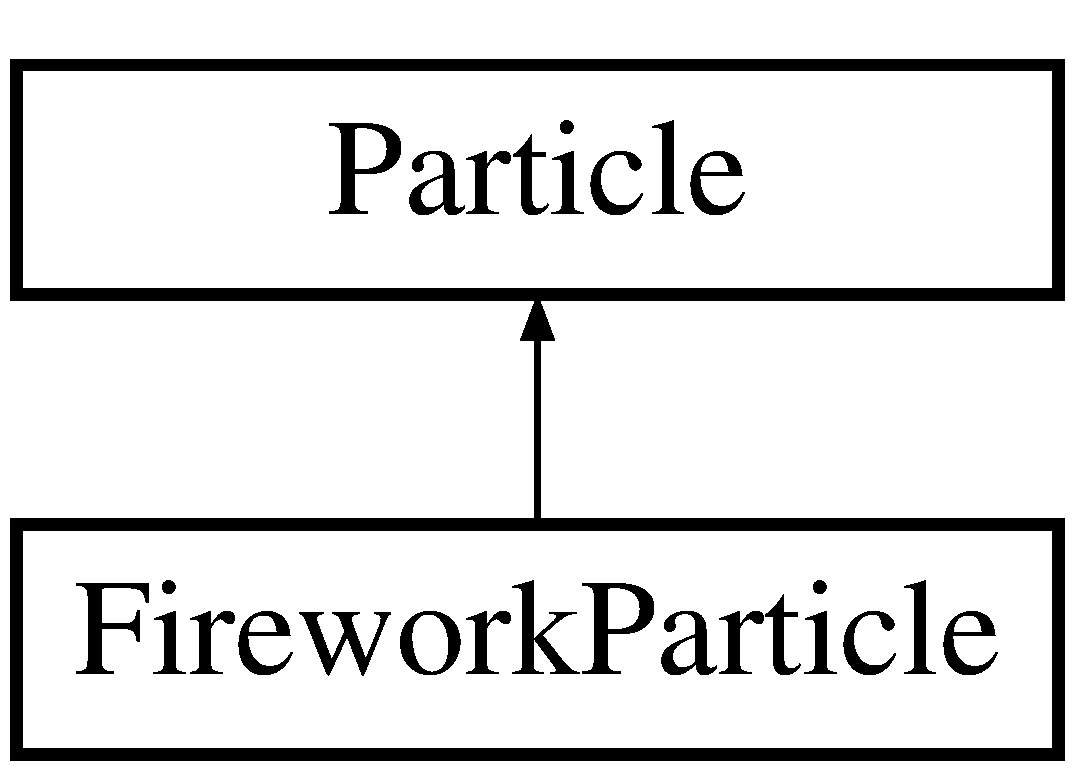
\includegraphics[height=2.000000cm]{classFireworkParticle}
\end{center}
\end{figure}
\subsection*{Public Member Functions}
\begin{DoxyCompactItemize}
\item 
\hypertarget{classFireworkParticle_a8900c1a99a0442e56dbff7153e967056}{\hyperlink{classFireworkParticle_a8900c1a99a0442e56dbff7153e967056}{Firework\-Particle} ()=default}\label{classFireworkParticle_a8900c1a99a0442e56dbff7153e967056}

\begin{DoxyCompactList}\small\item\em Default constructor that initialises member variables to default values. \end{DoxyCompactList}\item 
\hyperlink{classFireworkParticle_aa9833cf5c42acc247b734dbeb8125bc3}{Firework\-Particle} (int const \&\-\_\-fuse, glm\-::vec3 const \&\-\_\-pos, glm\-::vec3 const \&\-\_\-vel, glm\-::vec4 const \&\-\_\-col, float const \&\-\_\-brightness, float const \&\-\_\-size, int const \&\-\_\-life, int const \&\-\_\-elife, int const \&\-\_\-trail\-Life, int const \&\-\_\-frame, bool const \&\-\_\-spawn, bool const \&\-\_\-blink)
\begin{DoxyCompactList}\small\item\em Constructor using intial position, velocity, colour, size, life span and a spawn flag. \end{DoxyCompactList}\item 
\hypertarget{classFireworkParticle_a2093ec748627554a4e8b68663d4b2245}{virtual \hyperlink{classFireworkParticle_a2093ec748627554a4e8b68663d4b2245}{$\sim$\-Firework\-Particle} ()=default}\label{classFireworkParticle_a2093ec748627554a4e8b68663d4b2245}

\begin{DoxyCompactList}\small\item\em Default Virtual destructor for particle, neccessary to prevent memory leak. \end{DoxyCompactList}\item 
virtual int \hyperlink{classFireworkParticle_ac0149d0e10dc1e20d108354543f15299}{new\-Parts} (int const \&) const override
\begin{DoxyCompactList}\small\item\em Returns the amount of child particles to spawn, overrides the \hyperlink{classParticle}{Particle} class implementation. \end{DoxyCompactList}\item 
virtual void \hyperlink{classFireworkParticle_aacfe5d5991b4585c176d9e2315d0d293}{update} (int const \&\-\_\-frame) override
\begin{DoxyCompactList}\small\item\em Updates the particle properties, overrides the \hyperlink{classParticle}{Particle} class implementation. \end{DoxyCompactList}\item 
virtual void \hyperlink{classFireworkParticle_a495692a1f1f4a340c3d548215fd5e5d0}{draw} (int const \&\-\_\-frame) const override
\begin{DoxyCompactList}\small\item\em Draws the particle, overrides the \hyperlink{classParticle}{Particle} class implementation. \end{DoxyCompactList}\item 
virtual \hyperlink{classParticle}{Particle} $\ast$ \hyperlink{classFireworkParticle_a29256978e2558abb2fc808e3b96b8000}{create\-Child} (int const \&\-\_\-frame) const override
\begin{DoxyCompactList}\small\item\em Creates a pointer to a child particle, overrides the \hyperlink{classParticle}{Particle} class implementation. \end{DoxyCompactList}\end{DoxyCompactItemize}
\subsection*{Additional Inherited Members}


\subsection{Detailed Description}
encapsulates a firework particle, is derived from abstract \hyperlink{classParticle}{Particle} class 

Revision History\-: See \char`\"{}https\-://github.\-com/nitronoid/perfect\-Parts\char`\"{} Initial Version 20/03/17 

\subsection{Constructor \& Destructor Documentation}
\hypertarget{classFireworkParticle_aa9833cf5c42acc247b734dbeb8125bc3}{\index{Firework\-Particle@{Firework\-Particle}!Firework\-Particle@{Firework\-Particle}}
\index{Firework\-Particle@{Firework\-Particle}!FireworkParticle@{Firework\-Particle}}
\subsubsection[{Firework\-Particle}]{\setlength{\rightskip}{0pt plus 5cm}Firework\-Particle\-::\-Firework\-Particle (
\begin{DoxyParamCaption}
\item[{int const \&}]{\-\_\-fuse, }
\item[{glm\-::vec3 const \&}]{\-\_\-pos, }
\item[{glm\-::vec3 const \&}]{\-\_\-vel, }
\item[{glm\-::vec4 const \&}]{\-\_\-col, }
\item[{float const \&}]{\-\_\-brightness, }
\item[{float const \&}]{\-\_\-size, }
\item[{int const \&}]{\-\_\-life, }
\item[{int const \&}]{\-\_\-elife, }
\item[{int const \&}]{\-\_\-trail\-Life, }
\item[{int const \&}]{\-\_\-frame, }
\item[{bool const \&}]{\-\_\-spawn, }
\item[{bool const \&}]{\-\_\-blink}
\end{DoxyParamCaption}
)}}\label{classFireworkParticle_aa9833cf5c42acc247b734dbeb8125bc3}


Constructor using intial position, velocity, colour, size, life span and a spawn flag. 


\begin{DoxyParams}[1]{Parameters}
\mbox{\tt in}  & {\em \-\_\-fuse} & the amount of frames until the firework explodes \\
\hline
\mbox{\tt in}  & {\em \-\_\-pos} & the initial position of the particle \\
\hline
\mbox{\tt in}  & {\em \-\_\-vel} & the initial velocity of the particle \\
\hline
\mbox{\tt in}  & {\em \-\_\-col} & the initial colour of the particle \\
\hline
\mbox{\tt in}  & {\em \-\_\-brightness} & the intial brightness of the particle \\
\hline
\mbox{\tt in}  & {\em \-\_\-size} & the initial size of the particle \\
\hline
\mbox{\tt in}  & {\em \-\_\-life} & the initial life of the particle \\
\hline
\mbox{\tt in}  & {\em \-\_\-e\-Life} & the life of the particle after exploding \\
\hline
\mbox{\tt in}  & {\em \-\_\-trail\-Life} & the life span of child particles that compose trails \\
\hline
\mbox{\tt in}  & {\em \-\_\-frame} & the current frame, used to set m\-\_\-birth\-Frame \\
\hline
\mbox{\tt in}  & {\em \-\_\-spawn} & used to set m\-\_\-spawn, flag for spawning children \\
\hline
\mbox{\tt in}  & {\em \-\_\-blink} & used to set m\-\_\-blink, flag for blinking, or sparkling effect \\
\hline
\end{DoxyParams}


\subsection{Member Function Documentation}
\hypertarget{classFireworkParticle_a29256978e2558abb2fc808e3b96b8000}{\index{Firework\-Particle@{Firework\-Particle}!create\-Child@{create\-Child}}
\index{create\-Child@{create\-Child}!FireworkParticle@{Firework\-Particle}}
\subsubsection[{create\-Child}]{\setlength{\rightskip}{0pt plus 5cm}{\bf Particle} $\ast$ Firework\-Particle\-::create\-Child (
\begin{DoxyParamCaption}
\item[{int const \&}]{\-\_\-frame}
\end{DoxyParamCaption}
) const\hspace{0.3cm}{\ttfamily [override]}, {\ttfamily [virtual]}}}\label{classFireworkParticle_a29256978e2558abb2fc808e3b96b8000}


Creates a pointer to a child particle, overrides the \hyperlink{classParticle}{Particle} class implementation. 


\begin{DoxyParams}[1]{Parameters}
\mbox{\tt in}  & {\em \-\_\-frame} & the current frame \\
\hline
\end{DoxyParams}


Implements \hyperlink{classParticle_a3c7dcda6443a8cd16c142d6e712d3268}{Particle}.

\hypertarget{classFireworkParticle_a495692a1f1f4a340c3d548215fd5e5d0}{\index{Firework\-Particle@{Firework\-Particle}!draw@{draw}}
\index{draw@{draw}!FireworkParticle@{Firework\-Particle}}
\subsubsection[{draw}]{\setlength{\rightskip}{0pt plus 5cm}void Firework\-Particle\-::draw (
\begin{DoxyParamCaption}
\item[{int const \&}]{\-\_\-frame}
\end{DoxyParamCaption}
) const\hspace{0.3cm}{\ttfamily [override]}, {\ttfamily [virtual]}}}\label{classFireworkParticle_a495692a1f1f4a340c3d548215fd5e5d0}


Draws the particle, overrides the \hyperlink{classParticle}{Particle} class implementation. 


\begin{DoxyParams}[1]{Parameters}
\mbox{\tt in}  & {\em \-\_\-frame} & the current frame \\
\hline
\end{DoxyParams}


Implements \hyperlink{classParticle_a468fedc0c5773683ce0f14e7a906b184}{Particle}.

\hypertarget{classFireworkParticle_ac0149d0e10dc1e20d108354543f15299}{\index{Firework\-Particle@{Firework\-Particle}!new\-Parts@{new\-Parts}}
\index{new\-Parts@{new\-Parts}!FireworkParticle@{Firework\-Particle}}
\subsubsection[{new\-Parts}]{\setlength{\rightskip}{0pt plus 5cm}int Firework\-Particle\-::new\-Parts (
\begin{DoxyParamCaption}
\item[{int const \&}]{}
\end{DoxyParamCaption}
) const\hspace{0.3cm}{\ttfamily [override]}, {\ttfamily [virtual]}}}\label{classFireworkParticle_ac0149d0e10dc1e20d108354543f15299}


Returns the amount of child particles to spawn, overrides the \hyperlink{classParticle}{Particle} class implementation. 


\begin{DoxyParams}[1]{Parameters}
\mbox{\tt in}  & {\em parameter} & is unused, but required to allow polymorphism across all particles \\
\hline
\end{DoxyParams}


Implements \hyperlink{classParticle_abbaa24710a9341fe90df0da7b96a4014}{Particle}.

\hypertarget{classFireworkParticle_aacfe5d5991b4585c176d9e2315d0d293}{\index{Firework\-Particle@{Firework\-Particle}!update@{update}}
\index{update@{update}!FireworkParticle@{Firework\-Particle}}
\subsubsection[{update}]{\setlength{\rightskip}{0pt plus 5cm}void Firework\-Particle\-::update (
\begin{DoxyParamCaption}
\item[{int const \&}]{\-\_\-frame}
\end{DoxyParamCaption}
)\hspace{0.3cm}{\ttfamily [override]}, {\ttfamily [virtual]}}}\label{classFireworkParticle_aacfe5d5991b4585c176d9e2315d0d293}


Updates the particle properties, overrides the \hyperlink{classParticle}{Particle} class implementation. 


\begin{DoxyParams}[1]{Parameters}
\mbox{\tt in}  & {\em \-\_\-frame} & the current frame \\
\hline
\end{DoxyParams}


Reimplemented from \hyperlink{classParticle_a842b0304310e8e8e92119563bbefe8a9}{Particle}.



The documentation for this class was generated from the following files\-:\begin{DoxyCompactItemize}
\item 
include/\hyperlink{FireworkParticle_8h}{Firework\-Particle.\-h}\item 
src/\hyperlink{FireworkParticle_8cpp}{Firework\-Particle.\-cpp}\end{DoxyCompactItemize}

\hypertarget{classFlameParticle}{\section{Flame\-Particle Class Reference}
\label{classFlameParticle}\index{Flame\-Particle@{Flame\-Particle}}
}


encapsulates a flame particle, is derived from abstract \hyperlink{classParticle}{Particle} class  




{\ttfamily \#include $<$Flame\-Particle.\-h$>$}

Inheritance diagram for Flame\-Particle\-:\begin{figure}[H]
\begin{center}
\leavevmode
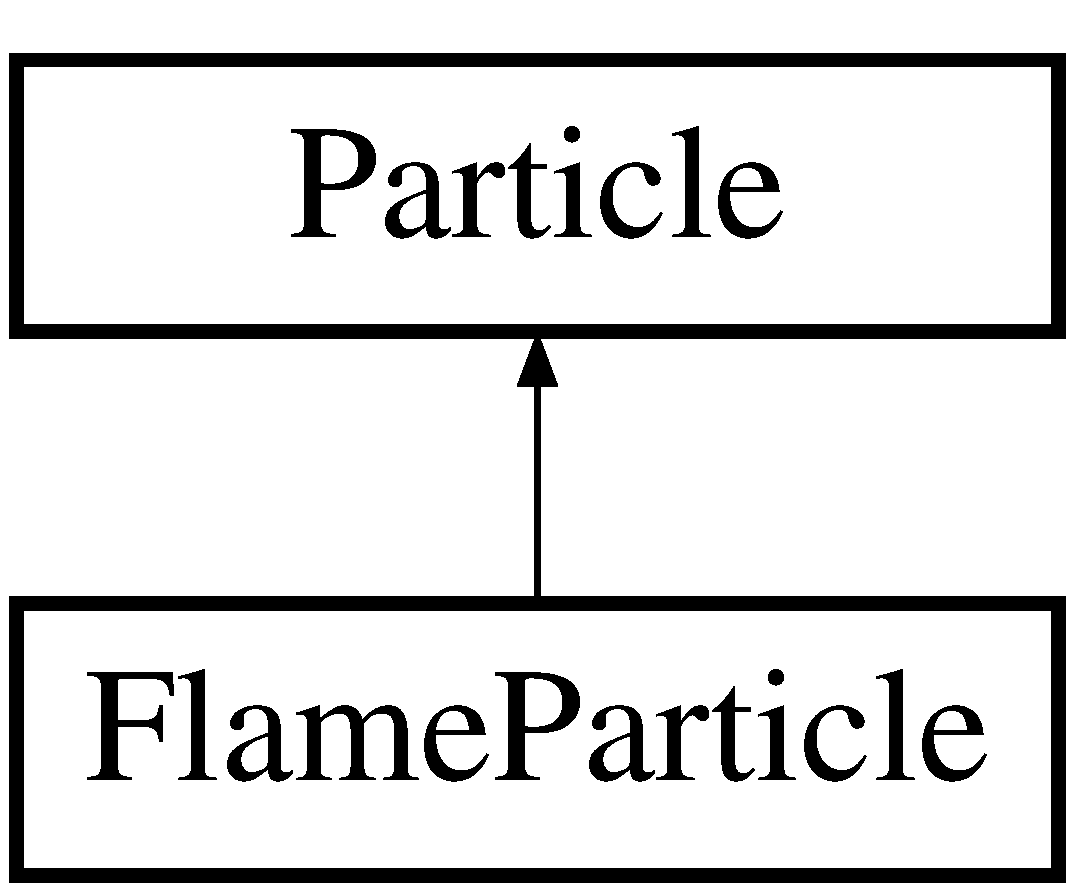
\includegraphics[height=2.000000cm]{classFlameParticle}
\end{center}
\end{figure}
\subsection*{Public Member Functions}
\begin{DoxyCompactItemize}
\item 
\hypertarget{classFlameParticle_af0faccc4ff4f1ff25aa1489cb98fee41}{\hyperlink{classFlameParticle_af0faccc4ff4f1ff25aa1489cb98fee41}{Flame\-Particle} ()=default}\label{classFlameParticle_af0faccc4ff4f1ff25aa1489cb98fee41}

\begin{DoxyCompactList}\small\item\em Default constructor that initialises member variables to default values. \end{DoxyCompactList}\item 
\hyperlink{classFlameParticle_aacb39d3f0127656555c0f5bdbf12dfea}{Flame\-Particle} (glm\-::vec3 const \&\-\_\-pos, glm\-::vec3 const \&\-\_\-vel, glm\-::vec4 const \&\-\_\-col, float const \&\-\_\-size, int const \&\-\_\-life, int const \&\-\_\-frame, bool const \&\-\_\-spawn)
\begin{DoxyCompactList}\small\item\em Constructor using intial position, velocity, colour, size, life span and a spawn flag. \end{DoxyCompactList}\item 
\hypertarget{classFlameParticle_a22bf84e45b0da08457b869be7671eb5b}{virtual \hyperlink{classFlameParticle_a22bf84e45b0da08457b869be7671eb5b}{$\sim$\-Flame\-Particle} ()=default}\label{classFlameParticle_a22bf84e45b0da08457b869be7671eb5b}

\begin{DoxyCompactList}\small\item\em Default Virtual destructor for particle, neccessary to prevent memory leak. \end{DoxyCompactList}\item 
virtual int \hyperlink{classFlameParticle_abe5fd489f2b08f16b6d2722be57c3f5c}{new\-Parts} (int const \&\-\_\-frame) const override
\begin{DoxyCompactList}\small\item\em Returns the amount of child particles to spawn, overrides the \hyperlink{classParticle}{Particle} class implementation. \end{DoxyCompactList}\item 
virtual void \hyperlink{classFlameParticle_a8d0b55a23c44197f404f707a04e1a5f3}{draw} (int const \&) const override
\begin{DoxyCompactList}\small\item\em Draws the particle, overrides the \hyperlink{classParticle}{Particle} class implementation. \end{DoxyCompactList}\item 
virtual \hyperlink{classParticle}{Particle} $\ast$ \hyperlink{classFlameParticle_aac20eda5440173cc4c2e7cd93a73eff0}{create\-Child} (int const \&\-\_\-frame) const override
\begin{DoxyCompactList}\small\item\em Creates a pointer to a child particle, overrides the \hyperlink{classParticle}{Particle} class implementation. \end{DoxyCompactList}\end{DoxyCompactItemize}
\subsection*{Additional Inherited Members}


\subsection{Detailed Description}
encapsulates a flame particle, is derived from abstract \hyperlink{classParticle}{Particle} class 

Revision History\-: See \char`\"{}https\-://github.\-com/nitronoid/perfect\-Parts\char`\"{} Initial Version 20/03/17 

\subsection{Constructor \& Destructor Documentation}
\hypertarget{classFlameParticle_aacb39d3f0127656555c0f5bdbf12dfea}{\index{Flame\-Particle@{Flame\-Particle}!Flame\-Particle@{Flame\-Particle}}
\index{Flame\-Particle@{Flame\-Particle}!FlameParticle@{Flame\-Particle}}
\subsubsection[{Flame\-Particle}]{\setlength{\rightskip}{0pt plus 5cm}Flame\-Particle\-::\-Flame\-Particle (
\begin{DoxyParamCaption}
\item[{glm\-::vec3 const \&}]{\-\_\-pos, }
\item[{glm\-::vec3 const \&}]{\-\_\-vel, }
\item[{glm\-::vec4 const \&}]{\-\_\-col, }
\item[{float const \&}]{\-\_\-size, }
\item[{int const \&}]{\-\_\-life, }
\item[{int const \&}]{\-\_\-frame, }
\item[{bool const \&}]{\-\_\-spawn}
\end{DoxyParamCaption}
)}}\label{classFlameParticle_aacb39d3f0127656555c0f5bdbf12dfea}


Constructor using intial position, velocity, colour, size, life span and a spawn flag. 


\begin{DoxyParams}[1]{Parameters}
\mbox{\tt in}  & {\em \-\_\-pos} & the initial position of the particle \\
\hline
\mbox{\tt in}  & {\em \-\_\-vel} & the initial velocity of the particle \\
\hline
\mbox{\tt in}  & {\em \-\_\-col} & the initial colour of the particle \\
\hline
\mbox{\tt in}  & {\em \-\_\-size} & the initial size of the particle \\
\hline
\mbox{\tt in}  & {\em \-\_\-life} & the initial life of the particle \\
\hline
\mbox{\tt in}  & {\em \-\_\-frame} & the current frame, used to set m\-\_\-birth\-Frame \\
\hline
\mbox{\tt in}  & {\em \-\_\-spawn} & used to set m\-\_\-spawn, flag for spawning children \\
\hline
\end{DoxyParams}


\subsection{Member Function Documentation}
\hypertarget{classFlameParticle_aac20eda5440173cc4c2e7cd93a73eff0}{\index{Flame\-Particle@{Flame\-Particle}!create\-Child@{create\-Child}}
\index{create\-Child@{create\-Child}!FlameParticle@{Flame\-Particle}}
\subsubsection[{create\-Child}]{\setlength{\rightskip}{0pt plus 5cm}{\bf Particle} $\ast$ Flame\-Particle\-::create\-Child (
\begin{DoxyParamCaption}
\item[{int const \&}]{\-\_\-frame}
\end{DoxyParamCaption}
) const\hspace{0.3cm}{\ttfamily [override]}, {\ttfamily [virtual]}}}\label{classFlameParticle_aac20eda5440173cc4c2e7cd93a73eff0}


Creates a pointer to a child particle, overrides the \hyperlink{classParticle}{Particle} class implementation. 


\begin{DoxyParams}[1]{Parameters}
\mbox{\tt in}  & {\em \-\_\-frame} & the current frame \\
\hline
\end{DoxyParams}


Implements \hyperlink{classParticle_a3c7dcda6443a8cd16c142d6e712d3268}{Particle}.

\hypertarget{classFlameParticle_a8d0b55a23c44197f404f707a04e1a5f3}{\index{Flame\-Particle@{Flame\-Particle}!draw@{draw}}
\index{draw@{draw}!FlameParticle@{Flame\-Particle}}
\subsubsection[{draw}]{\setlength{\rightskip}{0pt plus 5cm}void Flame\-Particle\-::draw (
\begin{DoxyParamCaption}
\item[{int const \&}]{}
\end{DoxyParamCaption}
) const\hspace{0.3cm}{\ttfamily [override]}, {\ttfamily [virtual]}}}\label{classFlameParticle_a8d0b55a23c44197f404f707a04e1a5f3}


Draws the particle, overrides the \hyperlink{classParticle}{Particle} class implementation. 


\begin{DoxyParams}[1]{Parameters}
\mbox{\tt in}  & {\em parameter} & is unused, but required to allow polymorphism across all particles \\
\hline
\end{DoxyParams}


Implements \hyperlink{classParticle_a468fedc0c5773683ce0f14e7a906b184}{Particle}.

\hypertarget{classFlameParticle_abe5fd489f2b08f16b6d2722be57c3f5c}{\index{Flame\-Particle@{Flame\-Particle}!new\-Parts@{new\-Parts}}
\index{new\-Parts@{new\-Parts}!FlameParticle@{Flame\-Particle}}
\subsubsection[{new\-Parts}]{\setlength{\rightskip}{0pt plus 5cm}int Flame\-Particle\-::new\-Parts (
\begin{DoxyParamCaption}
\item[{int const \&}]{\-\_\-frame}
\end{DoxyParamCaption}
) const\hspace{0.3cm}{\ttfamily [override]}, {\ttfamily [virtual]}}}\label{classFlameParticle_abe5fd489f2b08f16b6d2722be57c3f5c}


Returns the amount of child particles to spawn, overrides the \hyperlink{classParticle}{Particle} class implementation. 


\begin{DoxyParams}[1]{Parameters}
\mbox{\tt in}  & {\em \-\_\-frame} & the current frame \\
\hline
\end{DoxyParams}


Implements \hyperlink{classParticle_abbaa24710a9341fe90df0da7b96a4014}{Particle}.



The documentation for this class was generated from the following files\-:\begin{DoxyCompactItemize}
\item 
include/\hyperlink{FlameParticle_8h}{Flame\-Particle.\-h}\item 
src/Flame\-Particle.\-cpp\end{DoxyCompactItemize}

\hypertarget{classParticle}{\section{Particle Class Reference}
\label{classParticle}\index{Particle@{Particle}}
}


encapsulates a particle  




{\ttfamily \#include $<$Particle.\-h$>$}

Inheritance diagram for Particle\-:\begin{figure}[H]
\begin{center}
\leavevmode
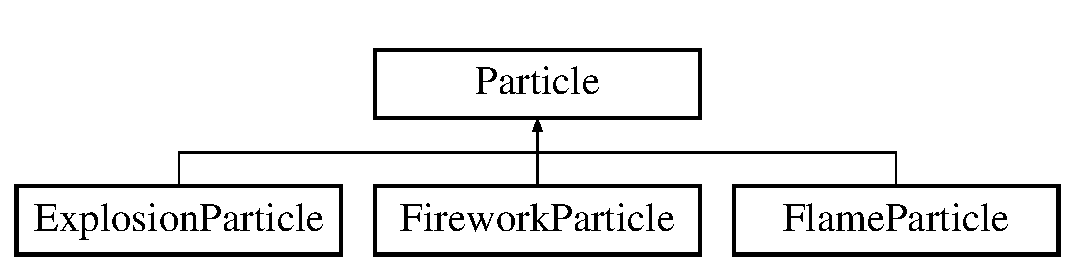
\includegraphics[height=2.000000cm]{classParticle}
\end{center}
\end{figure}
\subsection*{Public Member Functions}
\begin{DoxyCompactItemize}
\item 
\hypertarget{classParticle_a611ed46b6f07319f0e2f7bd588192a30}{\hyperlink{classParticle_a611ed46b6f07319f0e2f7bd588192a30}{Particle} ()=default}\label{classParticle_a611ed46b6f07319f0e2f7bd588192a30}

\begin{DoxyCompactList}\small\item\em Default constructor that initialises member variables to default values. \end{DoxyCompactList}\item 
\hyperlink{classParticle_abf90ea6b45c5e07a3945b1ac4b2b641d}{Particle} (glm\-::vec3 const \&\-\_\-pos, glm\-::vec3 const \&\-\_\-vel, glm\-::vec4 const \&\-\_\-col, float const \&\-\_\-size, int const \&\-\_\-life, int const \&\-\_\-frame, bool const \&\-\_\-spawn)
\begin{DoxyCompactList}\small\item\em Constructor using intial position, velocity, colour, size, life span and a spawn flag. \end{DoxyCompactList}\item 
\hypertarget{classParticle_a9d921eb3cc8673d98639bfc99c34da92}{virtual \hyperlink{classParticle_a9d921eb3cc8673d98639bfc99c34da92}{$\sim$\-Particle} ()=default}\label{classParticle_a9d921eb3cc8673d98639bfc99c34da92}

\begin{DoxyCompactList}\small\item\em Default Virtual destructor for particle, neccessary to prevent memory leak. \end{DoxyCompactList}\item 
virtual int \hyperlink{classParticle_abbaa24710a9341fe90df0da7b96a4014}{new\-Parts} (int const \&\-\_\-frame) const =0
\begin{DoxyCompactList}\small\item\em Returns the amount of child particles to spawn. \end{DoxyCompactList}\item 
virtual void \hyperlink{classParticle_a842b0304310e8e8e92119563bbefe8a9}{update} (int const \&)
\begin{DoxyCompactList}\small\item\em Updates the particle properties. \end{DoxyCompactList}\item 
virtual \hyperlink{classParticle}{Particle} $\ast$ \hyperlink{classParticle_a3c7dcda6443a8cd16c142d6e712d3268}{create\-Child} (int const \&\-\_\-frame) const =0
\begin{DoxyCompactList}\small\item\em Creates a pointer to a child particle. \end{DoxyCompactList}\item 
virtual void \hyperlink{classParticle_a468fedc0c5773683ce0f14e7a906b184}{draw} (int const \&\-\_\-frame) const =0
\begin{DoxyCompactList}\small\item\em Draws the particle. \end{DoxyCompactList}\end{DoxyCompactItemize}
\subsection*{Public Attributes}
\begin{DoxyCompactItemize}
\item 
\hypertarget{classParticle_afa6c5fb980874037e2ce0971f678b44d}{bool \hyperlink{classParticle_afa6c5fb980874037e2ce0971f678b44d}{m\-\_\-alive} = true}\label{classParticle_afa6c5fb980874037e2ce0971f678b44d}

\begin{DoxyCompactList}\small\item\em Flag telling us if the particle is currently alive. \end{DoxyCompactList}\item 
\hypertarget{classParticle_a1f7c4f4c38aa28b135d3b1abce3c0c02}{bool \hyperlink{classParticle_a1f7c4f4c38aa28b135d3b1abce3c0c02}{m\-\_\-spawn} = false}\label{classParticle_a1f7c4f4c38aa28b135d3b1abce3c0c02}

\begin{DoxyCompactList}\small\item\em Flag for whether or not this particle spawns children. \end{DoxyCompactList}\end{DoxyCompactItemize}
\subsection*{Protected Attributes}
\begin{DoxyCompactItemize}
\item 
\hypertarget{classParticle_a5583d126be9e5a2afa87d5696af7bc2d}{glm\-::vec3 \hyperlink{classParticle_a5583d126be9e5a2afa87d5696af7bc2d}{m\-\_\-pos} = glm\-::vec3(0.\-0f,0.\-0f,0.\-0f)}\label{classParticle_a5583d126be9e5a2afa87d5696af7bc2d}

\begin{DoxyCompactList}\small\item\em The position of the particle. \end{DoxyCompactList}\item 
\hypertarget{classParticle_a36b054c5a937be8d39b5b74e7c0ccaf2}{glm\-::vec3 \hyperlink{classParticle_a36b054c5a937be8d39b5b74e7c0ccaf2}{m\-\_\-vel} = glm\-::vec3(0.\-0f,0.\-0f,0.\-0f)}\label{classParticle_a36b054c5a937be8d39b5b74e7c0ccaf2}

\begin{DoxyCompactList}\small\item\em The velocity of the particle. \end{DoxyCompactList}\item 
\hypertarget{classParticle_acb820ee6efbbc886119bd322aabdbda5}{glm\-::vec3 \hyperlink{classParticle_acb820ee6efbbc886119bd322aabdbda5}{m\-\_\-accel} = glm\-::vec3(0.\-0f,-\/0.\-01f,0.\-0f)}\label{classParticle_acb820ee6efbbc886119bd322aabdbda5}

\begin{DoxyCompactList}\small\item\em The acceleration of the particle. \end{DoxyCompactList}\item 
\hypertarget{classParticle_a43e01bd0b50f845f9066b8efb574a4a0}{glm\-::vec4 \hyperlink{classParticle_a43e01bd0b50f845f9066b8efb574a4a0}{m\-\_\-col} = glm\-::vec4(1.\-0f,1.\-0f,1.\-0f,1.\-0f)}\label{classParticle_a43e01bd0b50f845f9066b8efb574a4a0}

\begin{DoxyCompactList}\small\item\em The colour of the particle. \end{DoxyCompactList}\item 
\hypertarget{classParticle_af28eb6fe8c29593ff02e0ecbd017c1ef}{glm\-::vec4 \hyperlink{classParticle_af28eb6fe8c29593ff02e0ecbd017c1ef}{m\-\_\-col\-Delta} = glm\-::vec4(0.\-0f,0.\-0f,0.\-0f,0.\-0f)}\label{classParticle_af28eb6fe8c29593ff02e0ecbd017c1ef}

\begin{DoxyCompactList}\small\item\em The rate of colour change. \end{DoxyCompactList}\item 
\hypertarget{classParticle_aa823a748fcec2f10bf44143389e4fae9}{G\-Lfloat \hyperlink{classParticle_aa823a748fcec2f10bf44143389e4fae9}{m\-\_\-size\-Delta} = 0.\-0f}\label{classParticle_aa823a748fcec2f10bf44143389e4fae9}

\begin{DoxyCompactList}\small\item\em The rate of size change. \end{DoxyCompactList}\item 
\hypertarget{classParticle_af6e8decb5f201ebabe1f460b0cfbbc8d}{G\-Lfloat \hyperlink{classParticle_af6e8decb5f201ebabe1f460b0cfbbc8d}{m\-\_\-size} = 5.\-0f}\label{classParticle_af6e8decb5f201ebabe1f460b0cfbbc8d}

\begin{DoxyCompactList}\small\item\em The size of the particle. \end{DoxyCompactList}\item 
\hypertarget{classParticle_a281390be9b1a6d0bf3c7506b01cae304}{int \hyperlink{classParticle_a281390be9b1a6d0bf3c7506b01cae304}{m\-\_\-life} = 100}\label{classParticle_a281390be9b1a6d0bf3c7506b01cae304}

\begin{DoxyCompactList}\small\item\em The remaining life span in frames. \end{DoxyCompactList}\item 
\hypertarget{classParticle_a86d093cab863dafaa67891f5fbcca8fc}{int \hyperlink{classParticle_a86d093cab863dafaa67891f5fbcca8fc}{m\-\_\-birth\-Frame} = 0}\label{classParticle_a86d093cab863dafaa67891f5fbcca8fc}

\begin{DoxyCompactList}\small\item\em The frame the particle was born. \end{DoxyCompactList}\end{DoxyCompactItemize}


\subsection{Detailed Description}
encapsulates a particle 

Revision History\-: See \char`\"{}https\-://github.\-com/nitronoid/perfect\-Parts\char`\"{} Initial Version 20/03/17 

\subsection{Constructor \& Destructor Documentation}
\hypertarget{classParticle_abf90ea6b45c5e07a3945b1ac4b2b641d}{\index{Particle@{Particle}!Particle@{Particle}}
\index{Particle@{Particle}!Particle@{Particle}}
\subsubsection[{Particle}]{\setlength{\rightskip}{0pt plus 5cm}Particle\-::\-Particle (
\begin{DoxyParamCaption}
\item[{glm\-::vec3 const \&}]{\-\_\-pos, }
\item[{glm\-::vec3 const \&}]{\-\_\-vel, }
\item[{glm\-::vec4 const \&}]{\-\_\-col, }
\item[{float const \&}]{\-\_\-size, }
\item[{int const \&}]{\-\_\-life, }
\item[{int const \&}]{\-\_\-frame, }
\item[{bool const \&}]{\-\_\-spawn}
\end{DoxyParamCaption}
)}}\label{classParticle_abf90ea6b45c5e07a3945b1ac4b2b641d}


Constructor using intial position, velocity, colour, size, life span and a spawn flag. 


\begin{DoxyParams}[1]{Parameters}
\mbox{\tt in}  & {\em \-\_\-pos} & the initial position of the particle \\
\hline
\mbox{\tt in}  & {\em \-\_\-vel} & the initial velocity of the particle \\
\hline
\mbox{\tt in}  & {\em \-\_\-col} & the initial colour of the particle \\
\hline
\mbox{\tt in}  & {\em \-\_\-size} & the initial size of the particle \\
\hline
\mbox{\tt in}  & {\em \-\_\-life} & the initial life of the particle \\
\hline
\mbox{\tt in}  & {\em \-\_\-frame} & the current frame, used to set m\-\_\-birth\-Frame \\
\hline
\mbox{\tt in}  & {\em \-\_\-spawn} & used to set m\-\_\-spawn, flag for spawning children \\
\hline
\end{DoxyParams}


\subsection{Member Function Documentation}
\hypertarget{classParticle_a3c7dcda6443a8cd16c142d6e712d3268}{\index{Particle@{Particle}!create\-Child@{create\-Child}}
\index{create\-Child@{create\-Child}!Particle@{Particle}}
\subsubsection[{create\-Child}]{\setlength{\rightskip}{0pt plus 5cm}virtual {\bf Particle}$\ast$ Particle\-::create\-Child (
\begin{DoxyParamCaption}
\item[{int const \&}]{\-\_\-frame}
\end{DoxyParamCaption}
) const\hspace{0.3cm}{\ttfamily [pure virtual]}}}\label{classParticle_a3c7dcda6443a8cd16c142d6e712d3268}


Creates a pointer to a child particle. 


\begin{DoxyParams}[1]{Parameters}
\mbox{\tt in}  & {\em \-\_\-frame} & the current frame \\
\hline
\end{DoxyParams}


Implemented in \hyperlink{classFireworkParticle_a29256978e2558abb2fc808e3b96b8000}{Firework\-Particle}, \hyperlink{classExplosionParticle_a1948c2b0f3b39d303b2d8cef6b0e0701}{Explosion\-Particle}, and \hyperlink{classFlameParticle_aac20eda5440173cc4c2e7cd93a73eff0}{Flame\-Particle}.

\hypertarget{classParticle_a468fedc0c5773683ce0f14e7a906b184}{\index{Particle@{Particle}!draw@{draw}}
\index{draw@{draw}!Particle@{Particle}}
\subsubsection[{draw}]{\setlength{\rightskip}{0pt plus 5cm}virtual void Particle\-::draw (
\begin{DoxyParamCaption}
\item[{int const \&}]{\-\_\-frame}
\end{DoxyParamCaption}
) const\hspace{0.3cm}{\ttfamily [pure virtual]}}}\label{classParticle_a468fedc0c5773683ce0f14e7a906b184}


Draws the particle. 


\begin{DoxyParams}[1]{Parameters}
\mbox{\tt in}  & {\em \-\_\-frame} & the current frame \\
\hline
\end{DoxyParams}


Implemented in \hyperlink{classFireworkParticle_a495692a1f1f4a340c3d548215fd5e5d0}{Firework\-Particle}, \hyperlink{classExplosionParticle_a0e3a9cd71e0d13732254f9184b7f38e9}{Explosion\-Particle}, and \hyperlink{classFlameParticle_a8d0b55a23c44197f404f707a04e1a5f3}{Flame\-Particle}.

\hypertarget{classParticle_abbaa24710a9341fe90df0da7b96a4014}{\index{Particle@{Particle}!new\-Parts@{new\-Parts}}
\index{new\-Parts@{new\-Parts}!Particle@{Particle}}
\subsubsection[{new\-Parts}]{\setlength{\rightskip}{0pt plus 5cm}virtual int Particle\-::new\-Parts (
\begin{DoxyParamCaption}
\item[{int const \&}]{\-\_\-frame}
\end{DoxyParamCaption}
) const\hspace{0.3cm}{\ttfamily [pure virtual]}}}\label{classParticle_abbaa24710a9341fe90df0da7b96a4014}


Returns the amount of child particles to spawn. 


\begin{DoxyParams}[1]{Parameters}
\mbox{\tt in}  & {\em \-\_\-frame} & the current frame \\
\hline
\end{DoxyParams}


Implemented in \hyperlink{classFireworkParticle_ac0149d0e10dc1e20d108354543f15299}{Firework\-Particle}, \hyperlink{classExplosionParticle_a302953be6e09fa22437248d175906e55}{Explosion\-Particle}, and \hyperlink{classFlameParticle_abe5fd489f2b08f16b6d2722be57c3f5c}{Flame\-Particle}.

\hypertarget{classParticle_a842b0304310e8e8e92119563bbefe8a9}{\index{Particle@{Particle}!update@{update}}
\index{update@{update}!Particle@{Particle}}
\subsubsection[{update}]{\setlength{\rightskip}{0pt plus 5cm}void Particle\-::update (
\begin{DoxyParamCaption}
\item[{int const \&}]{}
\end{DoxyParamCaption}
)\hspace{0.3cm}{\ttfamily [virtual]}}}\label{classParticle_a842b0304310e8e8e92119563bbefe8a9}


Updates the particle properties. 


\begin{DoxyParams}[1]{Parameters}
\mbox{\tt in}  & {\em parameter} & is unused, but required to allow polymorphism across all particles \\
\hline
\end{DoxyParams}


Reimplemented in \hyperlink{classFireworkParticle_aacfe5d5991b4585c176d9e2315d0d293}{Firework\-Particle}, and \hyperlink{classExplosionParticle_ac1c36920bf241f397c639fdaac40a9f9}{Explosion\-Particle}.



The documentation for this class was generated from the following files\-:\begin{DoxyCompactItemize}
\item 
include/\hyperlink{Particle_8h}{Particle.\-h}\item 
src/\hyperlink{Particle_8cpp}{Particle.\-cpp}\end{DoxyCompactItemize}

\hypertarget{classScene}{\section{Scene Class Reference}
\label{classScene}\index{Scene@{Scene}}
}


encapsulates a 3\-D Open\-G\-L \hyperlink{classScene}{Scene}  




{\ttfamily \#include $<$Scene.\-h$>$}

\subsection*{Public Member Functions}
\begin{DoxyCompactItemize}
\item 
\hypertarget{classScene_a93ccc41b0a2f6c24e467d5d9de76ec0d}{\hyperlink{classScene_a93ccc41b0a2f6c24e467d5d9de76ec0d}{Scene} ()=default}\label{classScene_a93ccc41b0a2f6c24e467d5d9de76ec0d}

\begin{DoxyCompactList}\small\item\em Default constructor that initialises member variables to default values. \end{DoxyCompactList}\item 
\hyperlink{classScene_acae65db27253defb67bb4a7f55dda339}{Scene} (std\-::string const \&\-\_\-name, int const \&\-\_\-x, int const \&\-\_\-y, int const \&\-\_\-width, int const \&\-\_\-height)
\begin{DoxyCompactList}\small\item\em Constructor that takes a name, intial size and intial position to generate an S\-D\-L window, with an Open\-G\-L context. \end{DoxyCompactList}\item 
\hypertarget{classScene_a6f6ba16bcbbf24d7f16df251b0a2ae3d}{\hyperlink{classScene_a6f6ba16bcbbf24d7f16df251b0a2ae3d}{Scene} (\hyperlink{classScene}{Scene} const \&)=delete}\label{classScene_a6f6ba16bcbbf24d7f16df251b0a2ae3d}

\begin{DoxyCompactList}\small\item\em Delete copy constructor, D\-O N\-O\-T I\-M\-P\-L\-E\-M\-E\-N\-T, emitter isn't trivially copyable. \end{DoxyCompactList}\item 
\hypertarget{classScene_a09aee6d6de84d1471e0300411e9d0df7}{\hyperlink{classScene}{Scene} \& \hyperlink{classScene_a09aee6d6de84d1471e0300411e9d0df7}{operator=} (\hyperlink{classScene}{Scene} const \&)=delete}\label{classScene_a09aee6d6de84d1471e0300411e9d0df7}

\begin{DoxyCompactList}\small\item\em Delete assignment, D\-O N\-O\-T I\-M\-P\-L\-E\-M\-E\-N\-T, emitter isn't trivially copyable. \end{DoxyCompactList}\item 
\hypertarget{classScene_a3b8cec2e32546713915f8c6303c951f1}{\hyperlink{classScene_a3b8cec2e32546713915f8c6303c951f1}{$\sim$\-Scene} ()}\label{classScene_a3b8cec2e32546713915f8c6303c951f1}

\begin{DoxyCompactList}\small\item\em Default destructor. \end{DoxyCompactList}\item 
\hypertarget{classScene_ab404b2cf95322ad5efd4f3f5d942bdaf}{void \hyperlink{classScene_ab404b2cf95322ad5efd4f3f5d942bdaf}{make\-Current} () const }\label{classScene_ab404b2cf95322ad5efd4f3f5d942bdaf}

\begin{DoxyCompactList}\small\item\em Calls S\-D\-L\-\_\-\-G\-L\-\_\-\-Make\-Current to link our S\-D\-L\-\_\-\-Window and Open\-G\-L context. \end{DoxyCompactList}\item 
\hypertarget{classScene_ac0e3d2c98ba6063a086467fb2c19142f}{void \hyperlink{classScene_ac0e3d2c98ba6063a086467fb2c19142f}{draw} ()}\label{classScene_ac0e3d2c98ba6063a086467fb2c19142f}

\begin{DoxyCompactList}\small\item\em Draws the G\-U\-I, particles and the window. \end{DoxyCompactList}\item 
\hypertarget{classScene_a839b81cdf0cdc807e48e660d92606496}{void \hyperlink{classScene_a839b81cdf0cdc807e48e660d92606496}{handle\-Input} ()}\label{classScene_a839b81cdf0cdc807e48e660d92606496}

\begin{DoxyCompactList}\small\item\em Handles user input, G\-U\-I, and manipulates emitter variables. \end{DoxyCompactList}\end{DoxyCompactItemize}
\subsection*{Public Attributes}
\begin{DoxyCompactItemize}
\item 
\hypertarget{classScene_a45e1e0091492b6012f5496a7bb16bc05}{bool \hyperlink{classScene_a45e1e0091492b6012f5496a7bb16bc05}{m\-\_\-quit} = false}\label{classScene_a45e1e0091492b6012f5496a7bb16bc05}

\begin{DoxyCompactList}\small\item\em Flag to close the window. \end{DoxyCompactList}\item 
\hypertarget{classScene_af6cba253a3657d48d17a6369a98a208b}{S\-D\-L\-\_\-\-Event \hyperlink{classScene_af6cba253a3657d48d17a6369a98a208b}{m\-\_\-input\-Event}}\label{classScene_af6cba253a3657d48d17a6369a98a208b}

\begin{DoxyCompactList}\small\item\em Holds the current user input. \end{DoxyCompactList}\end{DoxyCompactItemize}


\subsection{Detailed Description}
encapsulates a 3\-D Open\-G\-L \hyperlink{classScene}{Scene} 

Revision History\-: See \char`\"{}https\-://github.\-com/nitronoid/perfect\-Parts\char`\"{} Initial Version 20/03/17 \begin{DoxyRefDesc}{Todo}
\item[\hyperlink{todo__todo000002}{Todo}]extend G\-U\-I functionality \end{DoxyRefDesc}


\subsection{Constructor \& Destructor Documentation}
\hypertarget{classScene_acae65db27253defb67bb4a7f55dda339}{\index{Scene@{Scene}!Scene@{Scene}}
\index{Scene@{Scene}!Scene@{Scene}}
\subsubsection[{Scene}]{\setlength{\rightskip}{0pt plus 5cm}Scene\-::\-Scene (
\begin{DoxyParamCaption}
\item[{std\-::string const \&}]{\-\_\-name, }
\item[{int const \&}]{\-\_\-x, }
\item[{int const \&}]{\-\_\-y, }
\item[{int const \&}]{\-\_\-width, }
\item[{int const \&}]{\-\_\-height}
\end{DoxyParamCaption}
)}}\label{classScene_acae65db27253defb67bb4a7f55dda339}


Constructor that takes a name, intial size and intial position to generate an S\-D\-L window, with an Open\-G\-L context. 


\begin{DoxyParams}[1]{Parameters}
\mbox{\tt in}  & {\em \-\_\-name} & the name of the window \\
\hline
\mbox{\tt in}  & {\em \-\_\-x} & the intial x position of the window \\
\hline
\mbox{\tt in}  & {\em \-\_\-y} & the intial y position of the window \\
\hline
\mbox{\tt in}  & {\em \-\_\-width} & the intial width of the window \\
\hline
\mbox{\tt in}  & {\em \-\_\-height} & the intial height of the window \\
\hline
\end{DoxyParams}


The documentation for this class was generated from the following files\-:\begin{DoxyCompactItemize}
\item 
include/\hyperlink{Scene_8h}{Scene.\-h}\item 
src/Scene.\-cpp\end{DoxyCompactItemize}

\chapter{File Documentation}
\hypertarget{Emitter_8h}{\section{include/\-Emitter.h File Reference}
\label{Emitter_8h}\index{include/\-Emitter.\-h@{include/\-Emitter.\-h}}
}
{\ttfamily \#include $<$memory$>$}\\*
{\ttfamily \#include $<$vector$>$}\\*
{\ttfamily \#include $<$glm/glm.\-hpp$>$}\\*
{\ttfamily \#include $<$Q\-Dir$>$}\\*
{\ttfamily \#include \char`\"{}pngutils.\-h\char`\"{}}\\*
{\ttfamily \#include \char`\"{}Particle.\-h\char`\"{}}\\*
\subsection*{Classes}
\begin{DoxyCompactItemize}
\item 
class \hyperlink{classEmitter}{Emitter}
\begin{DoxyCompactList}\small\item\em encapsulates a particle emitter \end{DoxyCompactList}\end{DoxyCompactItemize}


\subsection{Detailed Description}
\begin{DoxyAuthor}{Author}
Jack Diver 
\end{DoxyAuthor}
\begin{DoxyVersion}{Version}
3.\-1 
\end{DoxyVersion}
\begin{DoxyDate}{Date}
Last Revision 03/05/17 Updated to N\-C\-C\-A coding standard \par
 
\end{DoxyDate}

\hypertarget{ExplosionParticle_8h}{\section{include/\-Explosion\-Particle.h File Reference}
\label{ExplosionParticle_8h}\index{include/\-Explosion\-Particle.\-h@{include/\-Explosion\-Particle.\-h}}
}
{\ttfamily \#include \char`\"{}Particle.\-h\char`\"{}}\\*
\subsection*{Classes}
\begin{DoxyCompactItemize}
\item 
class \hyperlink{classExplosionParticle}{Explosion\-Particle}
\begin{DoxyCompactList}\small\item\em encapsulates an explosion particle, is derived from abstract \hyperlink{classParticle}{Particle} class \end{DoxyCompactList}\end{DoxyCompactItemize}


\subsection{Detailed Description}
\begin{DoxyAuthor}{Author}
Jack Diver 
\end{DoxyAuthor}
\begin{DoxyVersion}{Version}
1.\-1 
\end{DoxyVersion}
\begin{DoxyDate}{Date}
Last Revision 03/05/17 Updated to N\-C\-C\-A coding standard \par
 
\end{DoxyDate}

\hypertarget{FireworkParticle_8h}{\section{include/\-Firework\-Particle.h File Reference}
\label{FireworkParticle_8h}\index{include/\-Firework\-Particle.\-h@{include/\-Firework\-Particle.\-h}}
}
{\ttfamily \#include \char`\"{}Particle.\-h\char`\"{}}\\*
\subsection*{Classes}
\begin{DoxyCompactItemize}
\item 
class \hyperlink{classFireworkParticle}{Firework\-Particle}
\begin{DoxyCompactList}\small\item\em encapsulates a firework particle, is derived from abstract \hyperlink{classParticle}{Particle} class \end{DoxyCompactList}\end{DoxyCompactItemize}


\subsection{Detailed Description}
\begin{DoxyAuthor}{Author}
Jack Diver 
\end{DoxyAuthor}
\begin{DoxyVersion}{Version}
2.\-1 
\end{DoxyVersion}
\begin{DoxyDate}{Date}
Last Revision 03/05/17 Updated to N\-C\-C\-A coding standard \par
 
\end{DoxyDate}

\hypertarget{FlameParticle_8h}{\section{include/\-Flame\-Particle.h File Reference}
\label{FlameParticle_8h}\index{include/\-Flame\-Particle.\-h@{include/\-Flame\-Particle.\-h}}
}
{\ttfamily \#include \char`\"{}Particle.\-h\char`\"{}}\\*
\subsection*{Classes}
\begin{DoxyCompactItemize}
\item 
class \hyperlink{classFlameParticle}{Flame\-Particle}
\begin{DoxyCompactList}\small\item\em encapsulates a flame particle, is derived from abstract \hyperlink{classParticle}{Particle} class \end{DoxyCompactList}\end{DoxyCompactItemize}


\subsection{Detailed Description}
\begin{DoxyAuthor}{Author}
Jack Diver 
\end{DoxyAuthor}
\begin{DoxyVersion}{Version}
3.\-4 
\end{DoxyVersion}
\begin{DoxyDate}{Date}
Last Revision 03/05/17 Updated to N\-C\-C\-A coding standard \par
 
\end{DoxyDate}

\hypertarget{Particle_8h}{\section{include/\-Particle.h File Reference}
\label{Particle_8h}\index{include/\-Particle.\-h@{include/\-Particle.\-h}}
}
{\ttfamily \#include $<$Open\-G\-L/gl.\-h$>$}\\*
{\ttfamily \#include $<$Open\-G\-L/glu.\-h$>$}\\*
{\ttfamily \#include $<$glm/glm.\-hpp$>$}\\*
\subsection*{Classes}
\begin{DoxyCompactItemize}
\item 
class \hyperlink{classParticle}{Particle}
\begin{DoxyCompactList}\small\item\em encapsulates a particle \end{DoxyCompactList}\end{DoxyCompactItemize}


\subsection{Detailed Description}
\begin{DoxyAuthor}{Author}
Jack Diver 
\end{DoxyAuthor}
\begin{DoxyVersion}{Version}
1.\-1 
\end{DoxyVersion}
\begin{DoxyDate}{Date}
Last Revision 03/05/17 Updated to N\-C\-C\-A coding standard \par
 
\end{DoxyDate}

\hypertarget{pngutils_8h}{\section{include/pngutils.h File Reference}
\label{pngutils_8h}\index{include/pngutils.\-h@{include/pngutils.\-h}}
}
{\ttfamily \#include $<$Open\-G\-L/gl.\-h$>$}\\*
{\ttfamily \#include $<$Open\-G\-L/glu.\-h$>$}\\*
\subsection*{Functions}
\begin{DoxyCompactItemize}
\item 
G\-Luint \hyperlink{pngutils_8h_a91be4e5fe91e8957390ee54b29fedb91}{png\-\_\-texture\-\_\-size} (const char $\ast$file\-\_\-name, G\-Luint \&width, G\-Luint \&height)
\begin{DoxyCompactList}\small\item\em Determine the width, height and raw data size of the png with the given filename. \end{DoxyCompactList}\item 
G\-Luint \hyperlink{pngutils_8h_a3e603317c013c990f2599cd986e0ebea}{png\-\_\-texture\-\_\-load} (const char $\ast$file\-\_\-name, G\-Lubyte $\ast$\&data)
\begin{DoxyCompactList}\small\item\em Load the image into the specified data. \end{DoxyCompactList}\item 
\hypertarget{pngutils_8h_ad2f510d17cd7d1606b496d6ea6c0b299}{bool \hyperlink{pngutils_8h_ad2f510d17cd7d1606b496d6ea6c0b299}{save\-\_\-png\-\_\-libpng} (const char $\ast$file\-\_\-name, uint8\-\_\-t $\ast$pixels, int w, int h)}\label{pngutils_8h_ad2f510d17cd7d1606b496d6ea6c0b299}

\begin{DoxyCompactList}\small\item\em Save frame buffer as .png image file. \end{DoxyCompactList}\end{DoxyCompactItemize}


\subsection{Detailed Description}
\begin{DoxyNote}{Note}
modified using pnglib code to allow saving a png \mbox{[}Accessed 2017\mbox{]}. Available from\-: \char`\"{}http\-://www.\-labbookpages.\-co.\-uk/software/img\-Proc/lib\-P\-N\-G.\-html\char`\"{} 
\end{DoxyNote}


\subsection{Function Documentation}
\hypertarget{pngutils_8h_a3e603317c013c990f2599cd986e0ebea}{\index{pngutils.\-h@{pngutils.\-h}!png\-\_\-texture\-\_\-load@{png\-\_\-texture\-\_\-load}}
\index{png\-\_\-texture\-\_\-load@{png\-\_\-texture\-\_\-load}!pngutils.h@{pngutils.\-h}}
\subsubsection[{png\-\_\-texture\-\_\-load}]{\setlength{\rightskip}{0pt plus 5cm}G\-Luint png\-\_\-texture\-\_\-load (
\begin{DoxyParamCaption}
\item[{const char $\ast$}]{file\-\_\-name, }
\item[{G\-Lubyte $\ast$\&}]{data}
\end{DoxyParamCaption}
)}}\label{pngutils_8h_a3e603317c013c990f2599cd986e0ebea}


Load the image into the specified data. 

Load the image into the specified data.


\begin{DoxyParams}{Parameters}
{\em file\-\_\-name} & The filename from which to load the data \\
\hline
{\em data} & The chunk of data to fill with this image \\
\hline
\end{DoxyParams}
\begin{DoxyReturn}{Returns}
E\-X\-I\-T\-\_\-\-S\-U\-C\-C\-E\-S\-S on success, E\-X\-I\-T\-\_\-\-F\-A\-I\-L\-U\-R\-E on failure 
\end{DoxyReturn}
\hypertarget{pngutils_8h_a91be4e5fe91e8957390ee54b29fedb91}{\index{pngutils.\-h@{pngutils.\-h}!png\-\_\-texture\-\_\-size@{png\-\_\-texture\-\_\-size}}
\index{png\-\_\-texture\-\_\-size@{png\-\_\-texture\-\_\-size}!pngutils.h@{pngutils.\-h}}
\subsubsection[{png\-\_\-texture\-\_\-size}]{\setlength{\rightskip}{0pt plus 5cm}G\-Luint png\-\_\-texture\-\_\-size (
\begin{DoxyParamCaption}
\item[{const char $\ast$}]{file\-\_\-name, }
\item[{G\-Luint \&}]{width, }
\item[{G\-Luint \&}]{height}
\end{DoxyParamCaption}
)}}\label{pngutils_8h_a91be4e5fe91e8957390ee54b29fedb91}


Determine the width, height and raw data size of the png with the given filename. 

Determine the width, height and raw data size of the png with the given filename.


\begin{DoxyParams}{Parameters}
{\em filename} & const char$\ast$ with name of texture filename \\
\hline
{\em width} & Passed by reference, set by this function if successful \\
\hline
{\em height} & Passed by reference, set by this function if successful \\
\hline
\end{DoxyParams}
\begin{DoxyReturn}{Returns}
0 on failure, or the size of the memory structure you need to malloc to load the image on success (raw) 
\end{DoxyReturn}

\hypertarget{Scene_8h}{\section{include/\-Scene.h File Reference}
\label{Scene_8h}\index{include/\-Scene.\-h@{include/\-Scene.\-h}}
}
{\ttfamily \#include $<$S\-D\-L.\-h$>$}\\*
{\ttfamily \#include $<$string$>$}\\*
{\ttfamily \#include $<$glm/glm.\-hpp$>$}\\*
{\ttfamily \#include \char`\"{}Emitter.\-h\char`\"{}}\\*
{\ttfamily \#include \char`\"{}Im\-G\-U\-I\-Impl.\-h\char`\"{}}\\*
\subsection*{Classes}
\begin{DoxyCompactItemize}
\item 
class \hyperlink{classScene}{Scene}
\begin{DoxyCompactList}\small\item\em encapsulates a 3\-D Open\-G\-L \hyperlink{classScene}{Scene} \end{DoxyCompactList}\end{DoxyCompactItemize}


\subsection{Detailed Description}
\begin{DoxyAuthor}{Author}
Jack Diver 
\end{DoxyAuthor}
\begin{DoxyVersion}{Version}
5.\-2 
\end{DoxyVersion}
\begin{DoxyDate}{Date}
Last Revision 03/05/17 Updated to N\-C\-C\-A coding standard \par
 
\end{DoxyDate}

\hypertarget{Emitter_8cpp}{\section{src/\-Emitter.cpp File Reference}
\label{Emitter_8cpp}\index{src/\-Emitter.\-cpp@{src/\-Emitter.\-cpp}}
}


Implementation files for \hyperlink{classEmitter}{Emitter} class.  


{\ttfamily \#include \char`\"{}Emitter.\-h\char`\"{}}\\*
{\ttfamily \#include \char`\"{}Flame\-Particle.\-h\char`\"{}}\\*
{\ttfamily \#include \char`\"{}Firework\-Particle.\-h\char`\"{}}\\*
{\ttfamily \#include \char`\"{}Explosion\-Particle.\-h\char`\"{}}\\*
{\ttfamily \#include $<$Q\-Image$>$}\\*
{\ttfamily \#include $<$Qt\-Open\-G\-L/\-Q\-G\-L\-Widget$>$}\\*
{\ttfamily \#include $<$glm/gtc/random.\-hpp$>$}\\*
{\ttfamily \#include $<$glm/gtc/type\-\_\-ptr.\-hpp$>$}\\*
{\ttfamily \#include $<$glm/gtx/fast\-\_\-trigonometry.\-hpp$>$}\\*
{\ttfamily \#include $<$chrono$>$}\\*
{\ttfamily \#include $<$iostream$>$}\\*


\subsection{Detailed Description}
Implementation files for \hyperlink{classEmitter}{Emitter} class. 
\hypertarget{ExplosionParticle_8cpp}{\section{src/\-Explosion\-Particle.cpp File Reference}
\label{ExplosionParticle_8cpp}\index{src/\-Explosion\-Particle.\-cpp@{src/\-Explosion\-Particle.\-cpp}}
}


Implementation files for Explosion \hyperlink{classParticle}{Particle} class.  


{\ttfamily \#include \char`\"{}Explosion\-Particle.\-h\char`\"{}}\\*
{\ttfamily \#include $<$glm/gtc/random.\-hpp$>$}\\*
{\ttfamily \#include $<$glm/gtc/type\-\_\-ptr.\-hpp$>$}\\*


\subsection{Detailed Description}
Implementation files for Explosion \hyperlink{classParticle}{Particle} class. 
\hypertarget{FireworkParticle_8cpp}{\section{src/\-Firework\-Particle.cpp File Reference}
\label{FireworkParticle_8cpp}\index{src/\-Firework\-Particle.\-cpp@{src/\-Firework\-Particle.\-cpp}}
}


Implementation files for Firework \hyperlink{classParticle}{Particle} class.  


{\ttfamily \#include \char`\"{}Firework\-Particle.\-h\char`\"{}}\\*
{\ttfamily \#include $<$glm/gtc/random.\-hpp$>$}\\*
{\ttfamily \#include $<$glm/gtc/type\-\_\-ptr.\-hpp$>$}\\*


\subsection{Detailed Description}
Implementation files for Firework \hyperlink{classParticle}{Particle} class. 
\hypertarget{main_8cpp}{\section{src/main.cpp File Reference}
\label{main_8cpp}\index{src/main.\-cpp@{src/main.\-cpp}}
}


Main function.  


{\ttfamily \#include $<$cstdlib$>$}\\*
{\ttfamily \#include \char`\"{}Scene.\-h\char`\"{}}\\*
\subsection*{Functions}
\begin{DoxyCompactItemize}
\item 
\hypertarget{main_8cpp_ae66f6b31b5ad750f1fe042a706a4e3d4}{int {\bfseries main} ()}\label{main_8cpp_ae66f6b31b5ad750f1fe042a706a4e3d4}

\end{DoxyCompactItemize}


\subsection{Detailed Description}
Main function. 
\hypertarget{Particle_8cpp}{\section{src/\-Particle.cpp File Reference}
\label{Particle_8cpp}\index{src/\-Particle.\-cpp@{src/\-Particle.\-cpp}}
}


Implementation files for \hyperlink{classParticle}{Particle} class.  


{\ttfamily \#include \char`\"{}Particle.\-h\char`\"{}}\\*


\subsection{Detailed Description}
Implementation files for \hyperlink{classParticle}{Particle} class. 
%--- End generated contents ---

% Index
\newpage
\phantomsection
\addcontentsline{toc}{part}{Index}
\printindex

\end{document}
